% STRATIA supplementary material, generated by scripts/supplementary.py from docs/data/*.md; do not edit.
% Build: pdflatex supp (no bibliography). Two-column for the title as the kit requires, one column after it.
\documentclass[10pt,twocolumn,letterpaper]{article}
\usepackage[review]{cvpr}
%% This file contains a number of tweaks that are typically applied to the main document.
%% They are not enabled by default, but can be enabled by uncommenting the relevant lines.


%%
%% Official support for 2-column teaser figure
%%
\usepackage{cuted} %< for strip environment

%%
%% For auto-referencing of figures (see fig/teaser.tex and \label{} therein) 
%%
\usepackage{currfile} %< for \currfilebase macro

%%
%% caption and (global) spacing overrides
%%
\usepackage{caption} %< for "\captionof" commands (teaser)
% \setlength{\abovecaptionskip}{.5em} % space above caption
% \setlength{\belowcaptionskip}{1em} % space below caption

%%
%% Inline annotations; for predefined colors, refer to "dvipsnames" in the xcolor package:
%% https://tinyurl.com/overleaf-colors
%%
\newcommand{\red}[1]{{\color{red}#1}}
\newcommand{\todo}[1]{{\color{red}#1}}
\newcommand{\TODO}[1]{\textbf{\color{red}[TODO: #1]}}
%%
%% Disable for camera ready / submission by uncommenting these lines:
%%
% \renewcommand{\TODO}[1]{}
% \renewcommand{\todo}[1]{#1}

%%
%% Work harder in optimizing text layout. Typically shrinks text by 1/6 of page, enable
%% it at the very end of the writing process, when you are just above the page limit.
%%
% \usepackage{microtype}

%%
%% Fine-tune paragraph spacing.
%%
% \renewcommand{\paragraph}[1]{\vspace{.5em}\noindent\textbf{#1.}}

%%
%% Globally adjusts space between figure and caption.
%%
% \setlength{\abovecaptionskip}{.5em}

%%
%% Allows "the use of \paper to refer to the project name"
%% with automatic management of space at the end of the word.
%%
% \usepackage{xspace}
% \newcommand{\paper}{ProjectName\xspace}

%%
%% Commonly used math definitions.
%%
% \DeclareMathOperator*{\argmin}{arg\,min}
% \DeclareMathOperator*{\argmax}{arg\,max}

%%
%% Tighten underline.
%%
% \usepackage{soul}
% \setuldepth{foobar}

%%
%% Reconfigure paragraph (tweaks spacing)
%%

\definecolor{cvprblue}{rgb}{0.21,0.49,0.74}
\usepackage[pagebackref,breaklinks,colorlinks,allcolors=cvprblue]{hyperref}
\def\confName{CVPR}
\def\confYear{2027}
\title{Supplementary Material for\\STRATIA: Honest Cloud Understanding from a Single Sky Camera}
\author{Anonymous \confName~submission\\}
\begin{document}
\maketitle
\onecolumn
\ifdefined\nolinenumbers\nolinenumbers\fi
\small
This supplement reproduces, in full, the result tables that the paper summarises: the one logged read of the locked
test sets (every model, split, metric and bootstrap interval), the ablations, the error analysis, the model as a
sixth annotator, the calibration, the robustness suite, the efficiency measurements, the Sun-track fit of the
authors' camera, and the data card of the collection. Every table was generated from the committed result files by
the released scripts; nothing here was typed by hand. The code, the split manifests, the lock file and the locked
results accompany this supplement.

\section{Locked-test results in full}

Split \texttt{test}; lock \texttt{c41841f43cc488d7}; run \texttt{20261025T113929Z\_locked\_test\_test\_f2f212f294}; git \texttt{7d4b7a4}; 500 cluster-bootstrap resamples; models and protocol as pre-registered in \texttt{docs/phases/P090-locked-test.md}. Thresholds 0.5; one seed except the in-domain global heads (three).

\subsection{The Gate G4 criteria on these rows}

{\scriptsize\setlength{\tabcolsep}{3pt}
\begin{longtable}{llllllll}
\toprule
Criterion & Quantity & P082 (val) & This split & 95 \% CI & Reference & Required & Holds \\
\midrule
\endhead
C1 & LODO étage macro-F1, mean of the four folds & 0.548 & 0.540 &  & 0.529 (probe ViT-B/16 @ 224, refitted) & $\geq$ reference + 0.05 & no \\
C1 & in-domain genus macro-F1 (CCSN, MGCD) & 0.719 & 0.706 &  & 0.733 (probe ViT-L/16 @ 224, refitted) & $\geq$ reference $-$ 0.01 & no \\
C2 & Montenegro étage-set agreement / human ceiling & 1.047 & 0.926 & [0.923, 0.928] & 0.900 (pre-registered bar) & $\geq$ 0.90 & yes \\
C2 & Montenegro oktas $\pm$1 agreement / human ceiling & 1.027 & 0.963 & [0.958, 0.966] & 0.900 (pre-registered bar) & $\geq$ 0.90 & yes \\
C3 & CBH skill, OLDLR (CDLRA) pairs & 0.471 & 0.536 & [0.440, 0.630] & 0.200 (pre-registered bar) & $\geq$ 0.20 & yes \\
C3 & CBH skill, WESTE (CDLRB) pairs, OLDLR-only training & 0.448 & 0.436 & [0.276, 0.585] & 0.100 (pre-registered bar) & $\geq$ 0.10 & yes \\
C3 & CBH MAE (m), all pairs, against the frozen-feature ridge & 566 & 872 & [679, 1055] & 1096 (ridge DINOv3 ViT-S/16 @ 512, refitted (the P058 CNN kept no checkpoint; 724 m on val)) & $\leq$ 0.9 $\times$ reference & yes \\
C3 & 80 \% interval coverage with the P089 temperature and radius & 0.802 & 0.720 &  & 0.800 (nominal) & 0.75–0.85 & no \\
\bottomrule
\end{longtable}}

\subsection{Every number}

\subsubsection{\texttt{in\_domain}}

{\scriptsize\setlength{\tabcolsep}{3pt}
\begin{longtable}{lllllll}
\toprule
Set & Model & Metric & Value & 95 \% CI & n & Note \\
\midrule
\endhead
almeria & \texttt{indomain\_e2s\_s0} & etage\_f1 & 0.803 & [0.678, 0.862] & 164 &  \\
almeria & \texttt{indomain\_e2s\_s0} & etage\_unsupported\_fp & - &  & 164 &  \\
almeria & \texttt{indomain\_e2s\_s0} & etage\_f1\_tuned & 0.815 & [0.726, 0.886] & 164 &  \\
almeria & \texttt{indomain\_e2s\_s0} & n\_etage & 164 & [116, 216] & 164 &  \\
ccsn & \texttt{indomain\_e2s\_s0} & etage\_f1 & 0.719 & [0.676, 0.756] & 512 &  \\
ccsn & \texttt{indomain\_e2s\_s0} & etage\_unsupported\_fp & - &  & 512 &  \\
ccsn & \texttt{indomain\_e2s\_s0} & etage\_f1\_tuned & 0.746 & [0.718, 0.785] & 512 &  \\
ccsn & \texttt{indomain\_e2s\_s0} & n\_etage & 512 & [502, 523] & 512 &  \\
ccsn & \texttt{indomain\_e2s\_s0} & genus\_f1 & 0.591 & [0.544, 0.629] & 512 &  \\
ccsn & \texttt{indomain\_e2s\_s0} & genus\_acc & 0.600 & [0.556, 0.643] & 512 &  \\
ccsn & \texttt{indomain\_e2s\_s0} & n\_genus & 512 & [502, 523] & 512 &  \\
mgcd & \texttt{indomain\_e2s\_s0} & etage\_f1 & 1.000 & [1.000, 1.000] & 1569 &  \\
mgcd & \texttt{indomain\_e2s\_s0} & etage\_unsupported\_fp & 0.000 & [0.000, 0.000] & 1569 &  \\
mgcd & \texttt{indomain\_e2s\_s0} & etage\_f1\_tuned & 1.000 & [1.000, 1.000] & 1569 &  \\
mgcd & \texttt{indomain\_e2s\_s0} & n\_etage & 816 & [291, 1380] & 1569 &  \\
mgcd & \texttt{indomain\_e2s\_s0} & genus\_f1 & 0.821 & [0.706, 0.997] & 1569 &  \\
mgcd & \texttt{indomain\_e2s\_s0} & genus\_acc & 0.879 & [0.648, 0.999] & 1569 &  \\
mgcd & \texttt{indomain\_e2s\_s0} & n\_genus & 1380 & [761, 2069] & 1569 &  \\
montenegro & \texttt{indomain\_e2s\_s0} & etage\_f1 & 0.680 & [0.629, 0.725] & 446 &  \\
montenegro & \texttt{indomain\_e2s\_s0} & etage\_unsupported\_fp & - &  & 446 &  \\
montenegro & \texttt{indomain\_e2s\_s0} & etage\_f1\_tuned & 0.700 & [0.696, 0.749] & 446 &  \\
montenegro & \texttt{indomain\_e2s\_s0} & n\_etage & 446 & [318, 574] & 446 &  \\
montenegro & \texttt{indomain\_e2s\_s0} & oktas\_mae & 0.706 & [0.648, 0.811] & 446 &  \\
montenegro & \texttt{indomain\_e2s\_s0} & oktas\_within1 & 0.841 & [0.836, 0.843] & 446 &  \\
montenegro & \texttt{indomain\_e2s\_s0} & oktas\_kl & 0.662 & [0.610, 0.757] & 446 &  \\
montenegro & \texttt{indomain\_e2s\_s0} & etage\_set\_agreement & 0.789 & [0.786, 0.791] & 446 &  \\
montenegro & \texttt{indomain\_e2s\_s0} & c2\_etage\_ratio & 0.926 & [0.923, 0.928] & 446 &  \\
montenegro & \texttt{indomain\_e2s\_s0} & c2\_oktas\_ratio & 0.963 & [0.958, 0.966] & 446 &  \\
almeria & \texttt{indomain\_e2s\_s1} & etage\_f1 & 0.801 &  & 164 &  \\
almeria & \texttt{indomain\_e2s\_s1} & etage\_unsupported\_fp & - &  & 164 &  \\
almeria & \texttt{indomain\_e2s\_s1} & etage\_f1\_tuned & 0.810 &  & 164 &  \\
almeria & \texttt{indomain\_e2s\_s1} & n\_etage & 164 &  & 164 &  \\
ccsn & \texttt{indomain\_e2s\_s1} & etage\_f1 & 0.732 &  & 512 &  \\
ccsn & \texttt{indomain\_e2s\_s1} & etage\_unsupported\_fp & - &  & 512 &  \\
ccsn & \texttt{indomain\_e2s\_s1} & etage\_f1\_tuned & 0.755 &  & 512 &  \\
ccsn & \texttt{indomain\_e2s\_s1} & n\_etage & 512 &  & 512 &  \\
ccsn & \texttt{indomain\_e2s\_s1} & genus\_f1 & 0.598 &  & 512 &  \\
ccsn & \texttt{indomain\_e2s\_s1} & genus\_acc & 0.611 &  & 512 &  \\
ccsn & \texttt{indomain\_e2s\_s1} & n\_genus & 512 &  & 512 &  \\
mgcd & \texttt{indomain\_e2s\_s1} & etage\_f1 & 1.000 &  & 1569 &  \\
mgcd & \texttt{indomain\_e2s\_s1} & etage\_unsupported\_fp & 0.000 &  & 1569 &  \\
mgcd & \texttt{indomain\_e2s\_s1} & etage\_f1\_tuned & 1.000 &  & 1569 &  \\
mgcd & \texttt{indomain\_e2s\_s1} & n\_etage & 816 &  & 1569 &  \\
mgcd & \texttt{indomain\_e2s\_s1} & genus\_f1 & 0.838 &  & 1569 &  \\
mgcd & \texttt{indomain\_e2s\_s1} & genus\_acc & 0.887 &  & 1569 &  \\
mgcd & \texttt{indomain\_e2s\_s1} & n\_genus & 1380 &  & 1569 &  \\
montenegro & \texttt{indomain\_e2s\_s1} & etage\_f1 & 0.664 &  & 446 &  \\
montenegro & \texttt{indomain\_e2s\_s1} & etage\_unsupported\_fp & - &  & 446 &  \\
montenegro & \texttt{indomain\_e2s\_s1} & etage\_f1\_tuned & 0.694 &  & 446 &  \\
montenegro & \texttt{indomain\_e2s\_s1} & n\_etage & 446 &  & 446 &  \\
montenegro & \texttt{indomain\_e2s\_s1} & oktas\_mae & 0.724 &  & 446 &  \\
montenegro & \texttt{indomain\_e2s\_s1} & oktas\_within1 & 0.839 &  & 446 &  \\
montenegro & \texttt{indomain\_e2s\_s1} & oktas\_kl & 0.657 &  & 446 &  \\
montenegro & \texttt{indomain\_e2s\_s1} & etage\_set\_agreement & 0.783 &  & 446 &  \\
montenegro & \texttt{indomain\_e2s\_s1} & c2\_etage\_ratio & 0.918 &  & 446 &  \\
montenegro & \texttt{indomain\_e2s\_s1} & c2\_oktas\_ratio & 0.961 &  & 446 &  \\
almeria & \texttt{indomain\_e2s\_s2} & etage\_f1 & 0.754 &  & 164 &  \\
almeria & \texttt{indomain\_e2s\_s2} & etage\_unsupported\_fp & - &  & 164 &  \\
almeria & \texttt{indomain\_e2s\_s2} & etage\_f1\_tuned & 0.797 &  & 164 &  \\
almeria & \texttt{indomain\_e2s\_s2} & n\_etage & 164 &  & 164 &  \\
ccsn & \texttt{indomain\_e2s\_s2} & etage\_f1 & 0.738 &  & 512 &  \\
ccsn & \texttt{indomain\_e2s\_s2} & etage\_unsupported\_fp & - &  & 512 &  \\
ccsn & \texttt{indomain\_e2s\_s2} & etage\_f1\_tuned & 0.749 &  & 512 &  \\
ccsn & \texttt{indomain\_e2s\_s2} & n\_etage & 512 &  & 512 &  \\
ccsn & \texttt{indomain\_e2s\_s2} & genus\_f1 & 0.593 &  & 512 &  \\
ccsn & \texttt{indomain\_e2s\_s2} & genus\_acc & 0.602 &  & 512 &  \\
ccsn & \texttt{indomain\_e2s\_s2} & n\_genus & 512 &  & 512 &  \\
mgcd & \texttt{indomain\_e2s\_s2} & etage\_f1 & 0.999 &  & 1569 &  \\
mgcd & \texttt{indomain\_e2s\_s2} & etage\_unsupported\_fp & 0.000 &  & 1569 &  \\
mgcd & \texttt{indomain\_e2s\_s2} & etage\_f1\_tuned & 1.000 &  & 1569 &  \\
mgcd & \texttt{indomain\_e2s\_s2} & n\_etage & 816 &  & 1569 &  \\
mgcd & \texttt{indomain\_e2s\_s2} & genus\_f1 & 0.826 &  & 1569 &  \\
mgcd & \texttt{indomain\_e2s\_s2} & genus\_acc & 0.880 &  & 1569 &  \\
mgcd & \texttt{indomain\_e2s\_s2} & n\_genus & 1380 &  & 1569 &  \\
montenegro & \texttt{indomain\_e2s\_s2} & etage\_f1 & 0.665 &  & 446 &  \\
montenegro & \texttt{indomain\_e2s\_s2} & etage\_unsupported\_fp & - &  & 446 &  \\
montenegro & \texttt{indomain\_e2s\_s2} & etage\_f1\_tuned & 0.704 &  & 446 &  \\
montenegro & \texttt{indomain\_e2s\_s2} & n\_etage & 446 &  & 446 &  \\
montenegro & \texttt{indomain\_e2s\_s2} & oktas\_mae & 0.697 &  & 446 &  \\
montenegro & \texttt{indomain\_e2s\_s2} & oktas\_within1 & 0.843 &  & 446 &  \\
montenegro & \texttt{indomain\_e2s\_s2} & oktas\_kl & 0.649 &  & 446 &  \\
montenegro & \texttt{indomain\_e2s\_s2} & etage\_set\_agreement & 0.780 &  & 446 &  \\
montenegro & \texttt{indomain\_e2s\_s2} & c2\_etage\_ratio & 0.916 &  & 446 &  \\
montenegro & \texttt{indomain\_e2s\_s2} & c2\_oktas\_ratio & 0.966 &  & 446 &  \\
almeria & \texttt{indomain\_e2s\_mean3} & etage\_f1 & 0.786 &  &  & std over 3 seeds 0.0226 \\
almeria & \texttt{indomain\_e2s\_mean3} & etage\_f1\_tuned & 0.807 &  &  & std over 3 seeds 0.0075 \\
almeria & \texttt{indomain\_e2s\_mean3} & n\_etage & 164 &  &  & std over 3 seeds 0.0000 \\
ccsn & \texttt{indomain\_e2s\_mean3} & etage\_f1 & 0.730 &  &  & std over 3 seeds 0.0080 \\
ccsn & \texttt{indomain\_e2s\_mean3} & etage\_f1\_tuned & 0.750 &  &  & std over 3 seeds 0.0036 \\
ccsn & \texttt{indomain\_e2s\_mean3} & genus\_acc & 0.604 &  &  & std over 3 seeds 0.0051 \\
ccsn & \texttt{indomain\_e2s\_mean3} & genus\_f1 & 0.594 &  &  & std over 3 seeds 0.0029 \\
ccsn & \texttt{indomain\_e2s\_mean3} & n\_etage & 512 &  &  & std over 3 seeds 0.0000 \\
ccsn & \texttt{indomain\_e2s\_mean3} & n\_genus & 512 &  &  & std over 3 seeds 0.0000 \\
mgcd & \texttt{indomain\_e2s\_mean3} & etage\_f1 & 1.000 &  &  & std over 3 seeds 0.0005 \\
mgcd & \texttt{indomain\_e2s\_mean3} & etage\_f1\_tuned & 1.000 &  &  & std over 3 seeds 0.0000 \\
mgcd & \texttt{indomain\_e2s\_mean3} & etage\_unsupported\_fp & 0.000 &  &  & std over 3 seeds 0.0000 \\
mgcd & \texttt{indomain\_e2s\_mean3} & genus\_acc & 0.882 &  &  & std over 3 seeds 0.0036 \\
mgcd & \texttt{indomain\_e2s\_mean3} & genus\_f1 & 0.828 &  &  & std over 3 seeds 0.0070 \\
mgcd & \texttt{indomain\_e2s\_mean3} & n\_etage & 816 &  &  & std over 3 seeds 0.0000 \\
mgcd & \texttt{indomain\_e2s\_mean3} & n\_genus & 1380 &  &  & std over 3 seeds 0.0000 \\
montenegro & \texttt{indomain\_e2s\_mean3} & c2\_etage\_ratio & 0.920 &  &  & std over 3 seeds 0.0045 \\
montenegro & \texttt{indomain\_e2s\_mean3} & c2\_oktas\_ratio & 0.963 &  &  & std over 3 seeds 0.0021 \\
montenegro & \texttt{indomain\_e2s\_mean3} & etage\_f1 & 0.670 &  &  & std over 3 seeds 0.0076 \\
montenegro & \texttt{indomain\_e2s\_mean3} & etage\_f1\_tuned & 0.699 &  &  & std over 3 seeds 0.0040 \\
montenegro & \texttt{indomain\_e2s\_mean3} & etage\_set\_agreement & 0.784 &  &  & std over 3 seeds 0.0038 \\
montenegro & \texttt{indomain\_e2s\_mean3} & n\_etage & 446 &  &  & std over 3 seeds 0.0000 \\
montenegro & \texttt{indomain\_e2s\_mean3} & oktas\_kl & 0.656 &  &  & std over 3 seeds 0.0054 \\
montenegro & \texttt{indomain\_e2s\_mean3} & oktas\_mae & 0.709 &  &  & std over 3 seeds 0.0112 \\
montenegro & \texttt{indomain\_e2s\_mean3} & oktas\_within1 & 0.841 &  &  & std over 3 seeds 0.0018 \\
ccsn & \texttt{probe\_dinov3\_vitl16\_224} & genus\_f1 & 0.549 & [0.501, 0.591] & 512 & C 0.01 chosen on val \\
ccsn & \texttt{probe\_dinov3\_vitl16\_224} & genus\_acc & 0.568 &  & 512 &  \\
mgcd & \texttt{probe\_dinov3\_vitl16\_224} & genus\_f1 & 0.918 & [0.763, 0.949] & 1569 & C 0.01 chosen on val \\
mgcd & \texttt{probe\_dinov3\_vitl16\_224} & genus\_acc & 0.930 &  & 1569 &  \\
\bottomrule
\end{longtable}}

\subsubsection{\texttt{cbh\_pairs\_etage}}

{\scriptsize\setlength{\tabcolsep}{3pt}
\begin{longtable}{lllllll}
\toprule
Set & Model & Metric & Value & 95 \% CI & n & Note \\
\midrule
\endhead
eye2sky\_cbh & \texttt{indomain\_e2s\_s0} & etage\_recall & 0.964 & [0.946, 0.984] & 2672 &  \\
eye2sky\_cbh & \texttt{indomain\_e2s\_s0} & lowest\_etage\_acc & 0.704 & [0.618, 0.778] & 2672 &  \\
eye2sky\_cbh & \texttt{indomain\_e2s\_s0} & n\_etage & 2672 & [2258, 3144] & 2672 &  \\
eye2sky\_cbh & \texttt{indomain\_e2s\_s1} & etage\_recall & 0.964 &  & 2672 &  \\
eye2sky\_cbh & \texttt{indomain\_e2s\_s1} & lowest\_etage\_acc & 0.713 &  & 2672 &  \\
eye2sky\_cbh & \texttt{indomain\_e2s\_s1} & n\_etage & 2672 &  & 2672 &  \\
eye2sky\_cbh & \texttt{indomain\_e2s\_s2} & etage\_recall & 0.962 &  & 2672 &  \\
eye2sky\_cbh & \texttt{indomain\_e2s\_s2} & lowest\_etage\_acc & 0.723 &  & 2672 &  \\
eye2sky\_cbh & \texttt{indomain\_e2s\_s2} & n\_etage & 2672 &  & 2672 &  \\
eye2sky\_cbh & \texttt{indomain\_e2s\_mean3} & etage\_recall & 0.963 &  &  & std over 3 seeds 0.0012 \\
eye2sky\_cbh & \texttt{indomain\_e2s\_mean3} & lowest\_etage\_acc & 0.714 &  &  & std over 3 seeds 0.0079 \\
eye2sky\_cbh & \texttt{indomain\_e2s\_mean3} & n\_etage & 2672 &  &  & std over 3 seeds 0.0000 \\
\bottomrule
\end{longtable}}

\subsubsection{\texttt{ood}}

{\scriptsize\setlength{\tabcolsep}{3pt}
\begin{longtable}{lllllll}
\toprule
Set & Model & Metric & Value & 95 \% CI & n & Note \\
\midrule
\endhead
in\_domain\_all & \texttt{indomain\_e2s\_s0} & flagged\_share & 0.054 &  & 5520 &  \\
almeria & \texttt{indomain\_e2s\_s0} & flagged\_share & 0.055 &  & 164 &  \\
ccsn & \texttt{indomain\_e2s\_s0} & flagged\_share & 0.430 &  & 512 &  \\
eye2sky & \texttt{indomain\_e2s\_s0} & flagged\_share & 0.000 &  & 2672 &  \\
mgcd & \texttt{indomain\_e2s\_s0} & flagged\_share & 0.022 &  & 1569 &  \\
montenegro & \texttt{indomain\_e2s\_s0} & flagged\_share & 0.004 &  & 446 &  \\
swim & \texttt{indomain\_e2s\_s0} & flagged\_share & 0.191 &  & 157 &  \\
b0268 & \texttt{indomain\_e2s\_s0} & flagged\_share & 0.400 &  & 120 &  \\
b0268\_vs\_in\_domain & \texttt{indomain\_e2s\_s0} & auroc & 0.939 &  & 5640 & higher score = out of domain; cached-feature path for both \\
\bottomrule
\end{longtable}}

\subsubsection{\texttt{lodo}}

{\scriptsize\setlength{\tabcolsep}{3pt}
\begin{longtable}{lllllll}
\toprule
Set & Model & Metric & Value & 95 \% CI & n & Note \\
\midrule
\endhead
ccsn & \texttt{lodo\_ccsn\_e2s} & etage\_f1 & 0.451 & [0.430, 0.471] & 2288 &  \\
ccsn & \texttt{lodo\_ccsn\_e2s} & etage\_unsupported\_fp & - &  & 2288 &  \\
ccsn & \texttt{lodo\_ccsn\_e2s} & etage\_f1\_tuned & 0.534 & [0.518, 0.553] & 2288 &  \\
ccsn & \texttt{lodo\_ccsn\_e2s} & n\_etage & 2109 & [2086, 2132] & 2288 &  \\
ccsn & \texttt{lodo\_ccsn\_e2s} & genus\_f1 & 0.091 & [0.081, 0.100] & 2288 &  \\
ccsn & \texttt{lodo\_ccsn\_e2s} & genus\_acc & 0.156 & [0.140, 0.171] & 2288 &  \\
ccsn & \texttt{lodo\_ccsn\_e2s} & n\_genus & 2288 & [2263, 2312] & 2288 &  \\
ccsn & \texttt{lodo\_ccsn\_e2s} & etage\_f1\_valtuned & 0.533 &  & 2109 & thresholds chosen on the fold's val rows \\
mgcd & \texttt{lodo\_mgcd\_e2s} & etage\_f1 & 0.709 & [0.620, 0.776] & 7041 &  \\
mgcd & \texttt{lodo\_mgcd\_e2s} & etage\_unsupported\_fp & 0.056 & [0.025, 0.097] & 7041 &  \\
mgcd & \texttt{lodo\_mgcd\_e2s} & etage\_f1\_tuned & 0.822 & [0.752, 0.875] & 7041 &  \\
mgcd & \texttt{lodo\_mgcd\_e2s} & n\_etage & 3661 & [2638, 4765] & 7041 &  \\
mgcd & \texttt{lodo\_mgcd\_e2s} & genus\_f1 & 0.517 & [0.443, 0.578] & 7041 &  \\
mgcd & \texttt{lodo\_mgcd\_e2s} & genus\_acc & 0.540 & [0.447, 0.627] & 7041 &  \\
mgcd & \texttt{lodo\_mgcd\_e2s} & n\_genus & 6191 & [4769, 7544] & 7041 &  \\
mgcd & \texttt{lodo\_mgcd\_e2s} & etage\_f1\_valtuned & 0.822 &  & 3661 & thresholds chosen on the fold's val rows \\
montenegro & \texttt{lodo\_montenegro\_e2s} & etage\_f1 & 0.367 & [0.298, 0.446] & 2011 &  \\
montenegro & \texttt{lodo\_montenegro\_e2s} & etage\_unsupported\_fp & - &  & 2011 &  \\
montenegro & \texttt{lodo\_montenegro\_e2s} & etage\_f1\_tuned & 0.492 & [0.426, 0.544] & 2011 &  \\
montenegro & \texttt{lodo\_montenegro\_e2s} & n\_etage & 2011 & [1720, 2288] & 2011 &  \\
montenegro & \texttt{lodo\_montenegro\_e2s} & oktas\_mae & 4.248 & [3.774, 4.829] & 2011 &  \\
montenegro & \texttt{lodo\_montenegro\_e2s} & oktas\_within1 & 0.311 & [0.249, 0.362] & 2011 &  \\
montenegro & \texttt{lodo\_montenegro\_e2s} & oktas\_kl & 1.645 & [1.575, 1.738] & 2011 &  \\
montenegro & \texttt{lodo\_montenegro\_e2s} & etage\_set\_agreement & 0.293 & [0.219, 0.381] & 2011 &  \\
montenegro & \texttt{lodo\_montenegro\_e2s} & c2\_etage\_ratio & 0.344 & [0.257, 0.448] & 2011 &  \\
montenegro & \texttt{lodo\_montenegro\_e2s} & c2\_oktas\_ratio & 0.357 & [0.285, 0.415] & 2011 &  \\
montenegro & \texttt{lodo\_montenegro\_e2s} & etage\_f1\_valtuned & 0.473 &  & 2011 & thresholds chosen on the fold's val rows \\
almeria & \texttt{lodo\_almeria\_e2s} & etage\_f1 & 0.634 & [0.599, 0.660] & 734 &  \\
almeria & \texttt{lodo\_almeria\_e2s} & etage\_unsupported\_fp & - &  & 734 &  \\
almeria & \texttt{lodo\_almeria\_e2s} & etage\_f1\_tuned & 0.646 & [0.620, 0.681] & 734 &  \\
almeria & \texttt{lodo\_almeria\_e2s} & n\_etage & 734 & [644, 832] & 734 &  \\
almeria & \texttt{lodo\_almeria\_e2s} & etage\_f1\_valtuned & 0.633 &  & 734 & thresholds chosen on the fold's val rows \\
ccsn & \texttt{probe\_dinov3\_vitb16\_224} & etage\_f1 & 0.396 & [0.376, 0.414] & 2109 & C 0.1 chosen on val \\
ccsn & \texttt{probe\_dinov3\_vitb16\_224} & etage\_unsupported\_fp & - &  & 2109 &  \\
mgcd & \texttt{probe\_dinov3\_vitb16\_224} & etage\_f1 & 0.860 & [0.793, 0.917] & 3661 & C 0.01 chosen on val \\
mgcd & \texttt{probe\_dinov3\_vitb16\_224} & etage\_unsupported\_fp & 0.009 &  & 3661 &  \\
montenegro & \texttt{probe\_dinov3\_vitb16\_224} & etage\_f1 & 0.463 & [0.392, 0.525] & 2011 & C 0.01 chosen on val \\
montenegro & \texttt{probe\_dinov3\_vitb16\_224} & etage\_unsupported\_fp & - &  & 2011 &  \\
almeria & \texttt{probe\_dinov3\_vitb16\_224} & etage\_f1 & 0.397 & [0.361, 0.425] & 734 & C 0.1 chosen on val \\
almeria & \texttt{probe\_dinov3\_vitb16\_224} & etage\_unsupported\_fp & - &  & 734 &  \\
\bottomrule
\end{longtable}}

\subsubsection{\texttt{dense}}

{\scriptsize\setlength{\tabcolsep}{3pt}
\begin{longtable}{lllllll}
\toprule
Set & Model & Metric & Value & 95 \% CI & n & Note \\
\midrule
\endhead
all & \texttt{dense\_sky\_layer\_s0} & sky\_miou & 0.900 & [0.897, 0.903] & 1775 &  \\
all & \texttt{dense\_sky\_layer\_s0} & iou\_invalid & 0.964 &  & 1775 &  \\
all & \texttt{dense\_sky\_layer\_s0} & iou\_sky & 0.859 &  & 1775 &  \\
all & \texttt{dense\_sky\_layer\_s0} & iou\_cloud & 0.878 &  & 1775 &  \\
all & \texttt{dense\_sky\_layer\_s0} & predicted\_cloud\_fraction & 0.528 &  & 1775 &  \\
all & \texttt{dense\_sky\_layer\_s0} & layer\_miou & 0.668 & [0.596, 0.743] & 1775 &  \\
all & \texttt{dense\_sky\_layer\_s0} & layer\_iou\_low & 0.783 &  & 1775 &  \\
all & \texttt{dense\_sky\_layer\_s0} & layer\_iou\_mid & 0.454 &  & 1775 &  \\
all & \texttt{dense\_sky\_layer\_s0} & layer\_iou\_high & 0.766 &  & 1775 &  \\
almeria & \texttt{dense\_sky\_layer\_s0} & sky\_miou & 0.885 & [0.871, 0.896] & 164 &  \\
almeria & \texttt{dense\_sky\_layer\_s0} & iou\_invalid & 0.964 &  & 164 &  \\
almeria & \texttt{dense\_sky\_layer\_s0} & iou\_sky & 0.867 &  & 164 &  \\
almeria & \texttt{dense\_sky\_layer\_s0} & iou\_cloud & 0.824 &  & 164 &  \\
almeria & \texttt{dense\_sky\_layer\_s0} & predicted\_cloud\_fraction & 0.335 &  & 164 &  \\
almeria & \texttt{dense\_sky\_layer\_s0} & layer\_miou & 0.668 & [0.597, 0.739] & 164 &  \\
almeria & \texttt{dense\_sky\_layer\_s0} & layer\_iou\_low & 0.783 &  & 164 &  \\
almeria & \texttt{dense\_sky\_layer\_s0} & layer\_iou\_mid & 0.454 &  & 164 &  \\
almeria & \texttt{dense\_sky\_layer\_s0} & layer\_iou\_high & 0.766 &  & 164 &  \\
shwimseg & \texttt{dense\_sky\_layer\_s0} & sky\_miou & 0.822 & [0.776, 0.860] & 31 &  \\
shwimseg & \texttt{dense\_sky\_layer\_s0} & iou\_sky & 0.806 &  & 31 &  \\
shwimseg & \texttt{dense\_sky\_layer\_s0} & iou\_cloud & 0.839 &  & 31 &  \\
shwimseg & \texttt{dense\_sky\_layer\_s0} & predicted\_cloud\_fraction & 0.553 &  & 31 &  \\
swimseg & \texttt{dense\_sky\_layer\_s0} & sky\_miou & 0.865 & [0.848, 0.879] & 203 &  \\
swimseg & \texttt{dense\_sky\_layer\_s0} & iou\_sky & 0.848 &  & 203 &  \\
swimseg & \texttt{dense\_sky\_layer\_s0} & iou\_cloud & 0.882 &  & 203 &  \\
swimseg & \texttt{dense\_sky\_layer\_s0} & predicted\_cloud\_fraction & 0.568 &  & 203 &  \\
swinseg & \texttt{dense\_sky\_layer\_s0} & sky\_miou & 0.866 & [0.840, 0.892] & 23 &  \\
swinseg & \texttt{dense\_sky\_layer\_s0} & iou\_sky & 0.867 &  & 23 &  \\
swinseg & \texttt{dense\_sky\_layer\_s0} & iou\_cloud & 0.865 &  & 23 &  \\
swinseg & \texttt{dense\_sky\_layer\_s0} & predicted\_cloud\_fraction & 0.497 &  & 23 &  \\
swinyseg & \texttt{dense\_sky\_layer\_s0} & sky\_miou & 0.872 & [0.866, 0.877] & 1354 &  \\
swinyseg & \texttt{dense\_sky\_layer\_s0} & iou\_sky & 0.861 &  & 1354 &  \\
swinyseg & \texttt{dense\_sky\_layer\_s0} & iou\_cloud & 0.883 &  & 1354 &  \\
swinyseg & \texttt{dense\_sky\_layer\_s0} & predicted\_cloud\_fraction & 0.546 &  & 1354 &  \\
clear\_sky\_test & \texttt{dense\_sky\_layer\_s0} & fraction\_invalid & 0.000 &  & 200 &  \\
clear\_sky\_test & \texttt{dense\_sky\_layer\_s0} & fraction\_sky & 0.719 &  & 200 &  \\
clear\_sky\_test & \texttt{dense\_sky\_layer\_s0} & fraction\_cloud & 0.281 &  & 200 &  \\
clear\_sky\_test & \texttt{dense\_sky\_layer\_s0} & fraction\_sun\_glare & 0.000 &  & 200 &  \\
\bottomrule
\end{longtable}}

\subsubsection{\texttt{cbh\_pairs}}

{\scriptsize\setlength{\tabcolsep}{3pt}
\begin{longtable}{lllllll}
\toprule
Set & Model & Metric & Value & 95 \% CI & n & Note \\
\midrule
\endhead
all & \texttt{climatology\_train} & mae\_m & 2012 &  & 2965 & clim 1726 m \\
all & \texttt{cbh\_base\_s0} & n & 2965 &  & 4383 &  \\
all & \texttt{cbh\_base\_s0} & mae\_m & 872 & [679, 1055] & 4383 &  \\
all & \texttt{cbh\_base\_s0} & bias\_m & -106 &  & 4383 &  \\
all & \texttt{cbh\_base\_s0} & rmsd\_m & 1524 &  & 4383 &  \\
all & \texttt{cbh\_base\_s0} & skill & 0.566 & [0.476, 0.663] & 4383 &  \\
all & \texttt{cbh\_base\_s0} & within\_250m & 0.363 &  & 4383 &  \\
all & \texttt{cbh\_base\_s0} & within\_500m & 0.546 & [0.456, 0.644] & 4383 &  \\
all & \texttt{cbh\_base\_s0} & within\_1000m & 0.747 &  & 4383 &  \\
all & \texttt{cbh\_base\_s0} & mae\_0-1000 & 339 &  & 4383 &  \\
all & \texttt{cbh\_base\_s0} & mae\_1000-2000 & 410 &  & 4383 &  \\
all & \texttt{cbh\_base\_s0} & mae\_2000-4000 & 853 &  & 4383 &  \\
all & \texttt{cbh\_base\_s0} & mae\_4000-8000 & 1785 &  & 4383 &  \\
all & \texttt{cbh\_base\_s0} & mae\_8000-20000 & 1923 &  & 4383 &  \\
all & \texttt{cbh\_base\_s0} & crps & 0.035 & [0.029, 0.041] & 4383 &  \\
all & \texttt{cbh\_base\_s0} & coverage\_80 & 0.878 & [0.847, 0.904] & 4383 &  \\
all & \texttt{cbh\_base\_s0} & cloud\_balanced\_acc & 0.915 &  & 4383 &  \\
all & \texttt{cbh\_base\_s0} & top\_bin\_share\_pred & 0.210 &  & 4383 &  \\
all & \texttt{cbh\_base\_s0} & top\_bin\_share\_true & 0.170 &  & 4383 &  \\
all & \texttt{cbh\_base\_s0} & entropy\_ratio & 0.903 &  & 4383 &  \\
all & \texttt{cbh\_base\_s0} & n\_cloudy & 2965 &  & 4383 &  \\
all & \texttt{cbh\_base\_s0} & coverage\_80\_calibrated & 0.720 &  & 2965 & P089 temperature 1.2394 and radius 0.3265 \\
all & \texttt{cbh\_base\_s0} & coverage\_95\_calibrated & 0.918 &  & 2965 & P089 temperature 1.2394 and radius 0.4376 \\
OLDLR & \texttt{cbh\_base\_s0} & n & 1466 &  & 2143 & skill against the training climatology's MAE on the whole split (Gate G4 definition) \\
OLDLR & \texttt{cbh\_base\_s0} & mae\_m & 933 & [744, 1127] & 2143 & skill against the training climatology's MAE on the whole split (Gate G4 definition) \\
OLDLR & \texttt{cbh\_base\_s0} & bias\_m & -46.408 &  & 2143 & skill against the training climatology's MAE on the whole split (Gate G4 definition) \\
OLDLR & \texttt{cbh\_base\_s0} & rmsd\_m & 1621 &  & 2143 & skill against the training climatology's MAE on the whole split (Gate G4 definition) \\
OLDLR & \texttt{cbh\_base\_s0} & skill & 0.536 & [0.440, 0.630] & 2143 & skill against the training climatology's MAE on the whole split (Gate G4 definition) \\
OLDLR & \texttt{cbh\_base\_s0} & within\_250m & 0.338 &  & 2143 & skill against the training climatology's MAE on the whole split (Gate G4 definition) \\
OLDLR & \texttt{cbh\_base\_s0} & within\_500m & 0.531 & [0.448, 0.618] & 2143 & skill against the training climatology's MAE on the whole split (Gate G4 definition) \\
OLDLR & \texttt{cbh\_base\_s0} & within\_1000m & 0.734 &  & 2143 & skill against the training climatology's MAE on the whole split (Gate G4 definition) \\
OLDLR & \texttt{cbh\_base\_s0} & mae\_0-1000 & 432 &  & 2143 & skill against the training climatology's MAE on the whole split (Gate G4 definition) \\
OLDLR & \texttt{cbh\_base\_s0} & mae\_1000-2000 & 449 &  & 2143 & skill against the training climatology's MAE on the whole split (Gate G4 definition) \\
OLDLR & \texttt{cbh\_base\_s0} & mae\_2000-4000 & 838 &  & 2143 & skill against the training climatology's MAE on the whole split (Gate G4 definition) \\
OLDLR & \texttt{cbh\_base\_s0} & mae\_4000-8000 & 1935 &  & 2143 & skill against the training climatology's MAE on the whole split (Gate G4 definition) \\
OLDLR & \texttt{cbh\_base\_s0} & mae\_8000-20000 & 1837 &  & 2143 & skill against the training climatology's MAE on the whole split (Gate G4 definition) \\
OLDLR & \texttt{cbh\_base\_s0} & crps & 0.038 & [0.032, 0.046] & 2143 & skill against the training climatology's MAE on the whole split (Gate G4 definition) \\
OLDLR & \texttt{cbh\_base\_s0} & coverage\_80 & 0.868 & [0.832, 0.900] & 2143 & skill against the training climatology's MAE on the whole split (Gate G4 definition) \\
OLDLR & \texttt{cbh\_base\_s0} & cloud\_balanced\_acc & 0.913 &  & 2143 & skill against the training climatology's MAE on the whole split (Gate G4 definition) \\
OLDLR & \texttt{cbh\_base\_s0} & top\_bin\_share\_pred & 0.236 &  & 2143 & skill against the training climatology's MAE on the whole split (Gate G4 definition) \\
OLDLR & \texttt{cbh\_base\_s0} & top\_bin\_share\_true & 0.158 &  & 2143 & skill against the training climatology's MAE on the whole split (Gate G4 definition) \\
OLDLR & \texttt{cbh\_base\_s0} & entropy\_ratio & 0.893 &  & 2143 & skill against the training climatology's MAE on the whole split (Gate G4 definition) \\
OLDLR & \texttt{cbh\_base\_s0} & n\_cloudy & 1466 &  & 2143 & skill against the training climatology's MAE on the whole split (Gate G4 definition) \\
OLDLR & \texttt{cbh\_base\_s0} & coverage\_80\_calibrated & 0.698 &  & 1466 & P089 temperature 1.2394 and radius 0.3265 \\
OLDLR & \texttt{cbh\_base\_s0} & coverage\_95\_calibrated & 0.911 &  & 1466 & P089 temperature 1.2394 and radius 0.4376 \\
OLDLR & \texttt{cbh\_base\_s0} & skill\_station\_climatology & 0.539 &  & 2143 & secondary: against the climatology's MAE on this station's rows (2024 m) \\
WESTE & \texttt{cbh\_base\_s0} & n & 1499 &  & 2240 & skill against the training climatology's MAE on the whole split (Gate G4 definition) \\
WESTE & \texttt{cbh\_base\_s0} & mae\_m & 813 & [601, 1013] & 2240 & skill against the training climatology's MAE on the whole split (Gate G4 definition) \\
WESTE & \texttt{cbh\_base\_s0} & bias\_m & -164 &  & 2240 & skill against the training climatology's MAE on the whole split (Gate G4 definition) \\
WESTE & \texttt{cbh\_base\_s0} & rmsd\_m & 1424 &  & 2240 & skill against the training climatology's MAE on the whole split (Gate G4 definition) \\
WESTE & \texttt{cbh\_base\_s0} & skill & 0.596 & [0.496, 0.701] & 2240 & skill against the training climatology's MAE on the whole split (Gate G4 definition) \\
WESTE & \texttt{cbh\_base\_s0} & within\_250m & 0.386 &  & 2240 & skill against the training climatology's MAE on the whole split (Gate G4 definition) \\
WESTE & \texttt{cbh\_base\_s0} & within\_500m & 0.561 & [0.458, 0.673] & 2240 & skill against the training climatology's MAE on the whole split (Gate G4 definition) \\
WESTE & \texttt{cbh\_base\_s0} & within\_1000m & 0.760 &  & 2240 & skill against the training climatology's MAE on the whole split (Gate G4 definition) \\
WESTE & \texttt{cbh\_base\_s0} & mae\_0-1000 & 249 &  & 2240 & skill against the training climatology's MAE on the whole split (Gate G4 definition) \\
WESTE & \texttt{cbh\_base\_s0} & mae\_1000-2000 & 376 &  & 2240 & skill against the training climatology's MAE on the whole split (Gate G4 definition) \\
WESTE & \texttt{cbh\_base\_s0} & mae\_2000-4000 & 869 &  & 2240 & skill against the training climatology's MAE on the whole split (Gate G4 definition) \\
WESTE & \texttt{cbh\_base\_s0} & mae\_4000-8000 & 1626 &  & 2240 & skill against the training climatology's MAE on the whole split (Gate G4 definition) \\
WESTE & \texttt{cbh\_base\_s0} & mae\_8000-20000 & 2004 &  & 2240 & skill against the training climatology's MAE on the whole split (Gate G4 definition) \\
WESTE & \texttt{cbh\_base\_s0} & crps & 0.032 & [0.026, 0.038] & 2240 & skill against the training climatology's MAE on the whole split (Gate G4 definition) \\
WESTE & \texttt{cbh\_base\_s0} & coverage\_80 & 0.887 & [0.855, 0.920] & 2240 & skill against the training climatology's MAE on the whole split (Gate G4 definition) \\
WESTE & \texttt{cbh\_base\_s0} & cloud\_balanced\_acc & 0.916 &  & 2240 & skill against the training climatology's MAE on the whole split (Gate G4 definition) \\
WESTE & \texttt{cbh\_base\_s0} & top\_bin\_share\_pred & 0.239 &  & 2240 & skill against the training climatology's MAE on the whole split (Gate G4 definition) \\
WESTE & \texttt{cbh\_base\_s0} & top\_bin\_share\_true & 0.183 &  & 2240 & skill against the training climatology's MAE on the whole split (Gate G4 definition) \\
WESTE & \texttt{cbh\_base\_s0} & entropy\_ratio & 0.905 &  & 2240 & skill against the training climatology's MAE on the whole split (Gate G4 definition) \\
WESTE & \texttt{cbh\_base\_s0} & n\_cloudy & 1499 &  & 2240 & skill against the training climatology's MAE on the whole split (Gate G4 definition) \\
WESTE & \texttt{cbh\_base\_s0} & coverage\_80\_calibrated & 0.742 &  & 1499 & P089 temperature 1.2394 and radius 0.3265 \\
WESTE & \texttt{cbh\_base\_s0} & coverage\_95\_calibrated & 0.925 &  & 1499 & P089 temperature 1.2394 and radius 0.4376 \\
WESTE & \texttt{cbh\_base\_s0} & skill\_station\_climatology & 0.593 &  & 2240 & secondary: against the climatology's MAE on this station's rows (1999 m) \\
all & \texttt{cbh\_base\_s0\_geometry\_zeroed} & n & 2965 &  & 4383 &  \\
all & \texttt{cbh\_base\_s0\_geometry\_zeroed} & mae\_m & 875 & [680, 1050] & 4383 &  \\
all & \texttt{cbh\_base\_s0\_geometry\_zeroed} & bias\_m & -11.869 &  & 4383 &  \\
all & \texttt{cbh\_base\_s0\_geometry\_zeroed} & rmsd\_m & 1526 &  & 4383 &  \\
all & \texttt{cbh\_base\_s0\_geometry\_zeroed} & skill & 0.565 & [0.478, 0.662] & 4383 &  \\
all & \texttt{cbh\_base\_s0\_geometry\_zeroed} & within\_250m & 0.354 &  & 4383 &  \\
all & \texttt{cbh\_base\_s0\_geometry\_zeroed} & within\_500m & 0.546 & [0.455, 0.651] & 4383 &  \\
all & \texttt{cbh\_base\_s0\_geometry\_zeroed} & within\_1000m & 0.741 &  & 4383 &  \\
all & \texttt{cbh\_base\_s0\_geometry\_zeroed} & mae\_0-1000 & 397 &  & 4383 &  \\
all & \texttt{cbh\_base\_s0\_geometry\_zeroed} & mae\_1000-2000 & 423 &  & 4383 &  \\
all & \texttt{cbh\_base\_s0\_geometry\_zeroed} & mae\_2000-4000 & 896 &  & 4383 &  \\
all & \texttt{cbh\_base\_s0\_geometry\_zeroed} & mae\_4000-8000 & 1740 &  & 4383 &  \\
all & \texttt{cbh\_base\_s0\_geometry\_zeroed} & mae\_8000-20000 & 1774 &  & 4383 &  \\
all & \texttt{cbh\_base\_s0\_geometry\_zeroed} & crps & 0.035 & [0.029, 0.040] & 4383 &  \\
all & \texttt{cbh\_base\_s0\_geometry\_zeroed} & coverage\_80 & 0.905 & [0.873, 0.928] & 4383 &  \\
all & \texttt{cbh\_base\_s0\_geometry\_zeroed} & cloud\_balanced\_acc & 0.910 &  & 4383 &  \\
all & \texttt{cbh\_base\_s0\_geometry\_zeroed} & top\_bin\_share\_pred & 0.234 &  & 4383 &  \\
all & \texttt{cbh\_base\_s0\_geometry\_zeroed} & top\_bin\_share\_true & 0.170 &  & 4383 &  \\
all & \texttt{cbh\_base\_s0\_geometry\_zeroed} & entropy\_ratio & 0.863 &  & 4383 &  \\
all & \texttt{cbh\_base\_s0\_geometry\_zeroed} & n\_cloudy & 2965 &  & 4383 &  \\
all & \texttt{cbh\_base\_s0\_geometry\_zeroed} & coverage\_80\_calibrated & 0.764 &  & 2965 & P089 temperature 1.2394 and radius 0.3265 \\
all & \texttt{cbh\_base\_s0\_geometry\_zeroed} & coverage\_95\_calibrated & 0.943 &  & 2965 & P089 temperature 1.2394 and radius 0.4376 \\
OLDLR & \texttt{cbh\_base\_s0\_geometry\_zeroed} & n & 1466 &  & 2143 & skill against the training climatology's MAE on the whole split (Gate G4 definition) \\
OLDLR & \texttt{cbh\_base\_s0\_geometry\_zeroed} & mae\_m & 941 & [746, 1129] & 2143 & skill against the training climatology's MAE on the whole split (Gate G4 definition) \\
OLDLR & \texttt{cbh\_base\_s0\_geometry\_zeroed} & bias\_m & 51.963 &  & 2143 & skill against the training climatology's MAE on the whole split (Gate G4 definition) \\
OLDLR & \texttt{cbh\_base\_s0\_geometry\_zeroed} & rmsd\_m & 1637 &  & 2143 & skill against the training climatology's MAE on the whole split (Gate G4 definition) \\
OLDLR & \texttt{cbh\_base\_s0\_geometry\_zeroed} & skill & 0.532 & [0.439, 0.629] & 2143 & skill against the training climatology's MAE on the whole split (Gate G4 definition) \\
OLDLR & \texttt{cbh\_base\_s0\_geometry\_zeroed} & within\_250m & 0.327 &  & 2143 & skill against the training climatology's MAE on the whole split (Gate G4 definition) \\
OLDLR & \texttt{cbh\_base\_s0\_geometry\_zeroed} & within\_500m & 0.529 & [0.441, 0.625] & 2143 & skill against the training climatology's MAE on the whole split (Gate G4 definition) \\
OLDLR & \texttt{cbh\_base\_s0\_geometry\_zeroed} & within\_1000m & 0.729 &  & 2143 & skill against the training climatology's MAE on the whole split (Gate G4 definition) \\
OLDLR & \texttt{cbh\_base\_s0\_geometry\_zeroed} & mae\_0-1000 & 528 &  & 2143 & skill against the training climatology's MAE on the whole split (Gate G4 definition) \\
OLDLR & \texttt{cbh\_base\_s0\_geometry\_zeroed} & mae\_1000-2000 & 458 &  & 2143 & skill against the training climatology's MAE on the whole split (Gate G4 definition) \\
OLDLR & \texttt{cbh\_base\_s0\_geometry\_zeroed} & mae\_2000-4000 & 881 &  & 2143 & skill against the training climatology's MAE on the whole split (Gate G4 definition) \\
OLDLR & \texttt{cbh\_base\_s0\_geometry\_zeroed} & mae\_4000-8000 & 1866 &  & 2143 & skill against the training climatology's MAE on the whole split (Gate G4 definition) \\
OLDLR & \texttt{cbh\_base\_s0\_geometry\_zeroed} & mae\_8000-20000 & 1720 &  & 2143 & skill against the training climatology's MAE on the whole split (Gate G4 definition) \\
OLDLR & \texttt{cbh\_base\_s0\_geometry\_zeroed} & crps & 0.038 & [0.032, 0.044] & 2143 & skill against the training climatology's MAE on the whole split (Gate G4 definition) \\
OLDLR & \texttt{cbh\_base\_s0\_geometry\_zeroed} & coverage\_80 & 0.901 & [0.867, 0.928] & 2143 & skill against the training climatology's MAE on the whole split (Gate G4 definition) \\
OLDLR & \texttt{cbh\_base\_s0\_geometry\_zeroed} & cloud\_balanced\_acc & 0.910 &  & 2143 & skill against the training climatology's MAE on the whole split (Gate G4 definition) \\
OLDLR & \texttt{cbh\_base\_s0\_geometry\_zeroed} & top\_bin\_share\_pred & 0.254 &  & 2143 & skill against the training climatology's MAE on the whole split (Gate G4 definition) \\
OLDLR & \texttt{cbh\_base\_s0\_geometry\_zeroed} & top\_bin\_share\_true & 0.158 &  & 2143 & skill against the training climatology's MAE on the whole split (Gate G4 definition) \\
OLDLR & \texttt{cbh\_base\_s0\_geometry\_zeroed} & entropy\_ratio & 0.855 &  & 2143 & skill against the training climatology's MAE on the whole split (Gate G4 definition) \\
OLDLR & \texttt{cbh\_base\_s0\_geometry\_zeroed} & n\_cloudy & 1466 &  & 2143 & skill against the training climatology's MAE on the whole split (Gate G4 definition) \\
OLDLR & \texttt{cbh\_base\_s0\_geometry\_zeroed} & coverage\_80\_calibrated & 0.744 &  & 1466 & P089 temperature 1.2394 and radius 0.3265 \\
OLDLR & \texttt{cbh\_base\_s0\_geometry\_zeroed} & coverage\_95\_calibrated & 0.935 &  & 1466 & P089 temperature 1.2394 and radius 0.4376 \\
OLDLR & \texttt{cbh\_base\_s0\_geometry\_zeroed} & skill\_station\_climatology & 0.535 &  & 2143 & secondary: against the climatology's MAE on this station's rows (2024 m) \\
WESTE & \texttt{cbh\_base\_s0\_geometry\_zeroed} & n & 1499 &  & 2240 & skill against the training climatology's MAE on the whole split (Gate G4 definition) \\
WESTE & \texttt{cbh\_base\_s0\_geometry\_zeroed} & mae\_m & 811 & [606, 1004] & 2240 & skill against the training climatology's MAE on the whole split (Gate G4 definition) \\
WESTE & \texttt{cbh\_base\_s0\_geometry\_zeroed} & bias\_m & -74.296 &  & 2240 & skill against the training climatology's MAE on the whole split (Gate G4 definition) \\
WESTE & \texttt{cbh\_base\_s0\_geometry\_zeroed} & rmsd\_m & 1408 &  & 2240 & skill against the training climatology's MAE on the whole split (Gate G4 definition) \\
WESTE & \texttt{cbh\_base\_s0\_geometry\_zeroed} & skill & 0.597 & [0.501, 0.699] & 2240 & skill against the training climatology's MAE on the whole split (Gate G4 definition) \\
WESTE & \texttt{cbh\_base\_s0\_geometry\_zeroed} & within\_250m & 0.382 &  & 2240 & skill against the training climatology's MAE on the whole split (Gate G4 definition) \\
WESTE & \texttt{cbh\_base\_s0\_geometry\_zeroed} & within\_500m & 0.564 & [0.461, 0.673] & 2240 & skill against the training climatology's MAE on the whole split (Gate G4 definition) \\
WESTE & \texttt{cbh\_base\_s0\_geometry\_zeroed} & within\_1000m & 0.754 &  & 2240 & skill against the training climatology's MAE on the whole split (Gate G4 definition) \\
WESTE & \texttt{cbh\_base\_s0\_geometry\_zeroed} & mae\_0-1000 & 272 &  & 2240 & skill against the training climatology's MAE on the whole split (Gate G4 definition) \\
WESTE & \texttt{cbh\_base\_s0\_geometry\_zeroed} & mae\_1000-2000 & 391 &  & 2240 & skill against the training climatology's MAE on the whole split (Gate G4 definition) \\
WESTE & \texttt{cbh\_base\_s0\_geometry\_zeroed} & mae\_2000-4000 & 912 &  & 2240 & skill against the training climatology's MAE on the whole split (Gate G4 definition) \\
WESTE & \texttt{cbh\_base\_s0\_geometry\_zeroed} & mae\_4000-8000 & 1606 &  & 2240 & skill against the training climatology's MAE on the whole split (Gate G4 definition) \\
WESTE & \texttt{cbh\_base\_s0\_geometry\_zeroed} & mae\_8000-20000 & 1825 &  & 2240 & skill against the training climatology's MAE on the whole split (Gate G4 definition) \\
WESTE & \texttt{cbh\_base\_s0\_geometry\_zeroed} & crps & 0.032 & [0.026, 0.037] & 2240 & skill against the training climatology's MAE on the whole split (Gate G4 definition) \\
WESTE & \texttt{cbh\_base\_s0\_geometry\_zeroed} & coverage\_80 & 0.909 & [0.881, 0.937] & 2240 & skill against the training climatology's MAE on the whole split (Gate G4 definition) \\
WESTE & \texttt{cbh\_base\_s0\_geometry\_zeroed} & cloud\_balanced\_acc & 0.911 &  & 2240 & skill against the training climatology's MAE on the whole split (Gate G4 definition) \\
WESTE & \texttt{cbh\_base\_s0\_geometry\_zeroed} & top\_bin\_share\_pred & 0.268 &  & 2240 & skill against the training climatology's MAE on the whole split (Gate G4 definition) \\
WESTE & \texttt{cbh\_base\_s0\_geometry\_zeroed} & top\_bin\_share\_true & 0.183 &  & 2240 & skill against the training climatology's MAE on the whole split (Gate G4 definition) \\
WESTE & \texttt{cbh\_base\_s0\_geometry\_zeroed} & entropy\_ratio & 0.862 &  & 2240 & skill against the training climatology's MAE on the whole split (Gate G4 definition) \\
WESTE & \texttt{cbh\_base\_s0\_geometry\_zeroed} & n\_cloudy & 1499 &  & 2240 & skill against the training climatology's MAE on the whole split (Gate G4 definition) \\
WESTE & \texttt{cbh\_base\_s0\_geometry\_zeroed} & coverage\_80\_calibrated & 0.783 &  & 1499 & P089 temperature 1.2394 and radius 0.3265 \\
WESTE & \texttt{cbh\_base\_s0\_geometry\_zeroed} & coverage\_95\_calibrated & 0.951 &  & 1499 & P089 temperature 1.2394 and radius 0.4376 \\
WESTE & \texttt{cbh\_base\_s0\_geometry\_zeroed} & skill\_station\_climatology & 0.595 &  & 2240 & secondary: against the climatology's MAE on this station's rows (1999 m) \\
WESTE & \texttt{cbh\_oldlr\_only\_s0} & n & 1499 &  & 2240 & site never seen in training; OLDLR training climatology (1750 m), its MAE on the whole split (Gate G4 definition) \\
WESTE & \texttt{cbh\_oldlr\_only\_s0} & mae\_m & 1134 & [835, 1456] & 2240 & site never seen in training; OLDLR training climatology (1750 m), its MAE on the whole split (Gate G4 definition) \\
WESTE & \texttt{cbh\_oldlr\_only\_s0} & bias\_m & -575 &  & 2240 & site never seen in training; OLDLR training climatology (1750 m), its MAE on the whole split (Gate G4 definition) \\
WESTE & \texttt{cbh\_oldlr\_only\_s0} & rmsd\_m & 1889 &  & 2240 & site never seen in training; OLDLR training climatology (1750 m), its MAE on the whole split (Gate G4 definition) \\
WESTE & \texttt{cbh\_oldlr\_only\_s0} & skill & 0.436 & [0.276, 0.585] & 2240 & site never seen in training; OLDLR training climatology (1750 m), its MAE on the whole split (Gate G4 definition) \\
WESTE & \texttt{cbh\_oldlr\_only\_s0} & within\_250m & 0.276 &  & 2240 & site never seen in training; OLDLR training climatology (1750 m), its MAE on the whole split (Gate G4 definition) \\
WESTE & \texttt{cbh\_oldlr\_only\_s0} & within\_500m & 0.496 & [0.403, 0.592] & 2240 & site never seen in training; OLDLR training climatology (1750 m), its MAE on the whole split (Gate G4 definition) \\
WESTE & \texttt{cbh\_oldlr\_only\_s0} & within\_1000m & 0.696 &  & 2240 & site never seen in training; OLDLR training climatology (1750 m), its MAE on the whole split (Gate G4 definition) \\
WESTE & \texttt{cbh\_oldlr\_only\_s0} & mae\_0-1000 & 364 &  & 2240 & site never seen in training; OLDLR training climatology (1750 m), its MAE on the whole split (Gate G4 definition) \\
WESTE & \texttt{cbh\_oldlr\_only\_s0} & mae\_1000-2000 & 501 &  & 2240 & site never seen in training; OLDLR training climatology (1750 m), its MAE on the whole split (Gate G4 definition) \\
WESTE & \texttt{cbh\_oldlr\_only\_s0} & mae\_2000-4000 & 868 &  & 2240 & site never seen in training; OLDLR training climatology (1750 m), its MAE on the whole split (Gate G4 definition) \\
WESTE & \texttt{cbh\_oldlr\_only\_s0} & mae\_4000-8000 & 1875 &  & 2240 & site never seen in training; OLDLR training climatology (1750 m), its MAE on the whole split (Gate G4 definition) \\
WESTE & \texttt{cbh\_oldlr\_only\_s0} & mae\_8000-20000 & 4214 &  & 2240 & site never seen in training; OLDLR training climatology (1750 m), its MAE on the whole split (Gate G4 definition) \\
WESTE & \texttt{cbh\_oldlr\_only\_s0} & crps & 0.049 & [0.040, 0.058] & 2240 & site never seen in training; OLDLR training climatology (1750 m), its MAE on the whole split (Gate G4 definition) \\
WESTE & \texttt{cbh\_oldlr\_only\_s0} & coverage\_80 & 0.799 & [0.754, 0.847] & 2240 & site never seen in training; OLDLR training climatology (1750 m), its MAE on the whole split (Gate G4 definition) \\
WESTE & \texttt{cbh\_oldlr\_only\_s0} & cloud\_balanced\_acc & 0.731 &  & 2240 & site never seen in training; OLDLR training climatology (1750 m), its MAE on the whole split (Gate G4 definition) \\
WESTE & \texttt{cbh\_oldlr\_only\_s0} & top\_bin\_share\_pred & 0.240 &  & 2240 & site never seen in training; OLDLR training climatology (1750 m), its MAE on the whole split (Gate G4 definition) \\
WESTE & \texttt{cbh\_oldlr\_only\_s0} & top\_bin\_share\_true & 0.183 &  & 2240 & site never seen in training; OLDLR training climatology (1750 m), its MAE on the whole split (Gate G4 definition) \\
WESTE & \texttt{cbh\_oldlr\_only\_s0} & entropy\_ratio & 0.819 &  & 2240 & site never seen in training; OLDLR training climatology (1750 m), its MAE on the whole split (Gate G4 definition) \\
WESTE & \texttt{cbh\_oldlr\_only\_s0} & n\_cloudy & 1499 &  & 2240 & site never seen in training; OLDLR training climatology (1750 m), its MAE on the whole split (Gate G4 definition) \\
WESTE & \texttt{cbh\_oldlr\_only\_s0} & coverage\_80\_calibrated & 0.605 &  & 1499 & P089 temperature 1.2394 and radius 0.3265 \\
WESTE & \texttt{cbh\_oldlr\_only\_s0} & coverage\_95\_calibrated & 0.855 &  & 1499 & P089 temperature 1.2394 and radius 0.4376 \\
WESTE & \texttt{cbh\_oldlr\_only\_s0} & skill\_station\_climatology & 0.433 &  & 2240 & secondary: against the OLDLR climatology's MAE on the WESTE rows (1999 m) \\
all & \texttt{ridge\_dinov3\_vits16\_512} & n & 2965 &  & 2965 & alpha 1000.0 chosen on val \\
all & \texttt{ridge\_dinov3\_vits16\_512} & mae\_m & 1096 & [852, 1365] & 2965 & alpha 1000.0 chosen on val \\
all & \texttt{ridge\_dinov3\_vits16\_512} & bias\_m & -285 &  & 2965 & alpha 1000.0 chosen on val \\
all & \texttt{ridge\_dinov3\_vits16\_512} & rmsd\_m & 1816 &  & 2965 & alpha 1000.0 chosen on val \\
all & \texttt{ridge\_dinov3\_vits16\_512} & skill & 0.455 &  & 2965 & alpha 1000.0 chosen on val \\
all & \texttt{ridge\_dinov3\_vits16\_512} & within\_250m & 0.295 &  & 2965 & alpha 1000.0 chosen on val \\
all & \texttt{ridge\_dinov3\_vits16\_512} & within\_500m & 0.470 &  & 2965 & alpha 1000.0 chosen on val \\
all & \texttt{ridge\_dinov3\_vits16\_512} & within\_1000m & 0.667 &  & 2965 & alpha 1000.0 chosen on val \\
all & \texttt{ridge\_dinov3\_vits16\_512} & mae\_0-1000 & 428 &  & 2965 & alpha 1000.0 chosen on val \\
all & \texttt{ridge\_dinov3\_vits16\_512} & mae\_1000-2000 & 472 &  & 2965 & alpha 1000.0 chosen on val \\
all & \texttt{ridge\_dinov3\_vits16\_512} & mae\_2000-4000 & 909 &  & 2965 & alpha 1000.0 chosen on val \\
all & \texttt{ridge\_dinov3\_vits16\_512} & mae\_4000-8000 & 2127 &  & 2965 & alpha 1000.0 chosen on val \\
all & \texttt{ridge\_dinov3\_vits16\_512} & mae\_8000-20000 & 3122 &  & 2965 & alpha 1000.0 chosen on val \\
OLDLR & \texttt{ridge\_dinov3\_vits16\_512} & n & 1466 &  & 1466 &  \\
OLDLR & \texttt{ridge\_dinov3\_vits16\_512} & mae\_m & 1117 &  & 1466 &  \\
OLDLR & \texttt{ridge\_dinov3\_vits16\_512} & bias\_m & -212 &  & 1466 &  \\
OLDLR & \texttt{ridge\_dinov3\_vits16\_512} & rmsd\_m & 1859 &  & 1466 &  \\
OLDLR & \texttt{ridge\_dinov3\_vits16\_512} & skill & 0.448 &  & 1466 &  \\
OLDLR & \texttt{ridge\_dinov3\_vits16\_512} & within\_250m & 0.286 &  & 1466 &  \\
OLDLR & \texttt{ridge\_dinov3\_vits16\_512} & within\_500m & 0.471 &  & 1466 &  \\
OLDLR & \texttt{ridge\_dinov3\_vits16\_512} & within\_1000m & 0.669 &  & 1466 &  \\
OLDLR & \texttt{ridge\_dinov3\_vits16\_512} & mae\_0-1000 & 467 &  & 1466 &  \\
OLDLR & \texttt{ridge\_dinov3\_vits16\_512} & mae\_1000-2000 & 491 &  & 1466 &  \\
OLDLR & \texttt{ridge\_dinov3\_vits16\_512} & mae\_2000-4000 & 894 &  & 1466 &  \\
OLDLR & \texttt{ridge\_dinov3\_vits16\_512} & mae\_4000-8000 & 2079 &  & 1466 &  \\
OLDLR & \texttt{ridge\_dinov3\_vits16\_512} & mae\_8000-20000 & 3187 &  & 1466 &  \\
WESTE & \texttt{ridge\_dinov3\_vits16\_512} & n & 1499 &  & 1499 &  \\
WESTE & \texttt{ridge\_dinov3\_vits16\_512} & mae\_m & 1075 &  & 1499 &  \\
WESTE & \texttt{ridge\_dinov3\_vits16\_512} & bias\_m & -356 &  & 1499 &  \\
WESTE & \texttt{ridge\_dinov3\_vits16\_512} & rmsd\_m & 1773 &  & 1499 &  \\
WESTE & \texttt{ridge\_dinov3\_vits16\_512} & skill & 0.462 &  & 1499 &  \\
WESTE & \texttt{ridge\_dinov3\_vits16\_512} & within\_250m & 0.304 &  & 1499 &  \\
WESTE & \texttt{ridge\_dinov3\_vits16\_512} & within\_500m & 0.469 &  & 1499 &  \\
WESTE & \texttt{ridge\_dinov3\_vits16\_512} & within\_1000m & 0.664 &  & 1499 &  \\
WESTE & \texttt{ridge\_dinov3\_vits16\_512} & mae\_0-1000 & 391 &  & 1499 &  \\
WESTE & \texttt{ridge\_dinov3\_vits16\_512} & mae\_1000-2000 & 456 &  & 1499 &  \\
WESTE & \texttt{ridge\_dinov3\_vits16\_512} & mae\_2000-4000 & 926 &  & 1499 &  \\
WESTE & \texttt{ridge\_dinov3\_vits16\_512} & mae\_4000-8000 & 2177 &  & 1499 &  \\
WESTE & \texttt{ridge\_dinov3\_vits16\_512} & mae\_8000-20000 & 3060 &  & 1499 &  \\
\bottomrule
\end{longtable}}

\subsubsection{\texttt{few\_shot\_target}}

{\scriptsize\setlength{\tabcolsep}{3pt}
\begin{longtable}{lllllll}
\toprule
Set & Model & Metric & Value & 95 \% CI & n & Note \\
\midrule
\endhead
locked\_day & \texttt{stratia-1.0.0-demo} & n & 120 &  & 120 &  \\
locked\_day & \texttt{stratia-1.0.0-demo} & etage\_set\_agreement & 0.000 &  & 120 &  \\
locked\_day & \texttt{stratia-1.0.0-demo} & c2\_etage\_ratio & 0.000 &  & 120 &  \\
locked\_day & \texttt{stratia-1.0.0-demo} & oktas\_within1 & 0.017 &  & 120 &  \\
locked\_day & \texttt{stratia-1.0.0-demo} & c2\_oktas\_ratio & 0.022 &  & 120 &  \\
locked\_day & \texttt{stratia-1.0.0-demo} & oktas\_mae & 3.458 &  & 120 &  \\
locked\_day & \texttt{stratia-1.0.0-demo} & oktas\_bias & 3.458 &  & 120 &  \\
locked\_day & \texttt{stratia-1.0.0-demo} & genus\_top1\_in\_set & 0.121 &  & 120 &  \\
locked\_day & \texttt{stratia-1.0.0-demo} & etage\_f1 & 0.217 &  & 120 &  \\
locked\_day & \texttt{stratia-1.0.0-demo} & cloud\_fraction\_corr\_vs\_cover & 0.776 &  & 120 &  \\
locked\_day & \texttt{stratia-1.0.0-demo} & cloud\_fraction\_mae\_vs\_cover & 0.079 &  & 120 &  \\
locked\_day & \texttt{stratia-1.0.0-demo} & glare\_fraction\_strong\_frames & 0.000 &  & 120 &  \\
locked\_day & \texttt{stratia-1.0.0-demo} & ood\_flagged\_share & 0.508 &  & 120 &  \\
locked\_day & \texttt{stratia-1.0.0-demo} & ood\_mean & 1.451 &  & 120 &  \\
locked\_day & \texttt{stratia-1.0.0-demo} & etage\_set\_agreement\_majority & 0.000 & [0.000, 0.000] & 120 & frame bootstrap, one day \\
locked\_day & \texttt{stratia-1.0.0-demo} & oktas\_within1\_majority & 0.000 & [0.000, 0.000] & 120 & frame bootstrap, one day \\
locked\_day & \texttt{stratia-1.0.1-demo} & n & 120 &  & 120 &  \\
locked\_day & \texttt{stratia-1.0.1-demo} & etage\_set\_agreement & 0.463 &  & 120 &  \\
locked\_day & \texttt{stratia-1.0.1-demo} & c2\_etage\_ratio & 0.508 &  & 120 &  \\
locked\_day & \texttt{stratia-1.0.1-demo} & oktas\_within1 & 0.671 &  & 120 &  \\
locked\_day & \texttt{stratia-1.0.1-demo} & c2\_oktas\_ratio & 0.870 &  & 120 &  \\
locked\_day & \texttt{stratia-1.0.1-demo} & oktas\_mae & 1.000 &  & 120 &  \\
locked\_day & \texttt{stratia-1.0.1-demo} & oktas\_bias & -0.500 &  & 120 &  \\
locked\_day & \texttt{stratia-1.0.1-demo} & genus\_top1\_in\_set & 1.000 &  & 120 &  \\
locked\_day & \texttt{stratia-1.0.1-demo} & etage\_f1 & 0.821 &  & 120 &  \\
locked\_day & \texttt{stratia-1.0.1-demo} & cloud\_fraction\_corr\_vs\_cover & 0.776 &  & 120 &  \\
locked\_day & \texttt{stratia-1.0.1-demo} & cloud\_fraction\_mae\_vs\_cover & 0.079 &  & 120 &  \\
locked\_day & \texttt{stratia-1.0.1-demo} & glare\_fraction\_strong\_frames & 0.000 &  & 120 &  \\
locked\_day & \texttt{stratia-1.0.1-demo} & ood\_flagged\_share & 0.000 &  & 120 &  \\
locked\_day & \texttt{stratia-1.0.1-demo} & ood\_mean & 0.832 &  & 120 &  \\
locked\_day & \texttt{stratia-1.0.1-demo} & etage\_set\_agreement\_majority & 0.458 & [0.375, 0.546] & 120 & frame bootstrap, one day \\
locked\_day & \texttt{stratia-1.0.1-demo} & oktas\_within1\_majority & 0.900 & [0.842, 0.950] & 120 & frame bootstrap, one day \\
\bottomrule
\end{longtable}}

Not evaluated (no model exists): \texttt{lodo/swim/test}, \texttt{held\_out\_station/same\_days/test}, \texttt{held\_out\_station/disjoint\_days/test}.


\section{Ablations}

Every row is a validation number read from the Stage H result tables or the five P091 runs; the reference is the Gate G4 configuration. Global rows: mean étage macro-F1 over the sources and mean genus macro-F1 (CCSN, MGCD, SWIMCAT), the Montenegro C2 ratios and the Eye2Sky lowest-étage accuracy; one seed each, the reference's spread over three seeds is étage $\pm$ nan, genus $\pm$ nan. Backbone size was not ablated: only 224-px CLS caches exist for ViT-B/L (the P054 probes stand in); augmentation does not apply to heads trained on cached features (P080 covers regularisation). Not retrained here; the locked test (P090) was read once and is not touched.

\subsection{Global heads}

\begin{center}{\scriptsize\setlength{\tabcolsep}{3pt}
\begin{tabular}{lp{3.0cm}llllll}
\toprule
Group & Variant & Étage F1 ($\Delta$) & Genus F1 ($\Delta$) & C2 étage ratio & C2 oktas ratio & Eye2Sky lowest-étage acc & Run \\
\midrule
reference & Gate G4 heads (geometry dropout 0.3, soft and set-valued targets, hierarchy loss 0.1, Eye2Sky étage rows) & 0.817 (+0.000) & 0.719 (+0.000) & - & - & - & \texttt{20261011T125754Z} \\
geometry (SkyRay) & no geometry: ray map and Sun always dropped (p\_drop 1.0) & 0.809 (-0.008) & 0.720 (+0.001) & - & - & - & \texttt{20261105T134909Z} \\
geometry (SkyRay) & geometry always given (p\_drop 0.0) & 0.829 (+0.011) & 0.709 (-0.010) & - & - & - & \texttt{20261105T135443Z} \\
targets & hard targets: first listed genus, majority étages, majority okta & 0.794 (-0.023) & 0.729 (+0.010) & - & - & - & \texttt{20261105T135923Z} \\
loss & no hierarchy loss (lambda\_h 0) & 0.813 (-0.005) & 0.712 (-0.007) & - & - & - & \texttt{20261105T140344Z} \\
loss & uncertainty (Kendall) task weighting & 0.814 (-0.003) & 0.716 (-0.002) & - & - & - & \texttt{20261105T140931Z} \\
Eye2Sky étage rows & without the ceilometer étage rows (indomain) & 0.823 (+0.005) & 0.738 (+0.019) & - & - & - & \texttt{20261011T100505Z} \\
regularisation (P080) & head dropout 0 & 0.804 (-0.013) & 0.703 (-0.016) & - & - & - & \texttt{20261011T122932Z} \\
regularisation (P080) & head dropout 0.3 & 0.817 (-0.000) & 0.743 (+0.024) & - & - & - & \texttt{20261011T123353Z} \\
regularisation (P080) & weight decay 0 & 0.816 (-0.001) & 0.722 (+0.004) & - & - & - & \texttt{20261011T121812Z} \\
regularisation (P080) & weight decay 0.2 & 0.815 (-0.002) & 0.715 (-0.004) & - & - & - & \texttt{20261011T122312Z} \\
regularisation (P080) & no EMA & 0.820 (+0.003) & 0.711 (-0.008) & - & - & - & \texttt{20261011T123824Z} \\
regularisation (P080) & EMA 0.999 & 0.812 (-0.006) & 0.708 (-0.011) & - & - & - & \texttt{20261011T124318Z} \\
\bottomrule
\end{tabular}}
\end{center}

\begin{center}{\scriptsize\setlength{\tabcolsep}{3pt}
\begin{tabular}{lll}
\toprule
LODO fold & Variant & Held-out étage F1 \\
\midrule
held-out ccsn & with Eye2Sky étage rows & 0.489 \\
held-out ccsn & without & 0.486 \\
held-out mgcd & with Eye2Sky étage rows & 0.749 \\
held-out mgcd & without & 0.871 \\
held-out montenegro & with Eye2Sky étage rows & 0.360 \\
held-out montenegro & without & 0.258 \\
held-out almeria & with Eye2Sky étage rows & 0.593 \\
held-out almeria & without & 0.327 \\
\bottomrule
\end{tabular}}
\end{center}

\subsection{multi-task (P076)}

\begin{center}{\scriptsize\setlength{\tabcolsep}{3pt}
\begin{tabular}{lllll}
\toprule
Variant & mean\_etage\_f1 & sky\_miou & layer\_miou & cbh\_mae\_m \\
\midrule
joint training: joint & 0.812 & - & 0.544 & - \\
joint training: joint\_long & 0.799 & - & 0.421 & - \\
\bottomrule
\end{tabular}}
\end{center}

\subsection{partial unfreeze (P077)}

\begin{center}{\scriptsize\setlength{\tabcolsep}{3pt}
\begin{tabular}{p{11.4cm}lll}
\toprule
Variant & mean\_etage\_f1 & mean\_etage\_f1\_before & mean\_genus\_f1 \\
\midrule
LoRA: lora (after / before) & 0.810 & 0.805 & - \\
LoRA: lora\_lowhead (after / before) & 0.810 & 0.805 & - \\
\bottomrule
\end{tabular}}
\end{center}

\subsection{CBH head (P075)}

\begin{center}{\scriptsize\setlength{\tabcolsep}{3pt}
\begin{tabular}{p{12.7cm}lll}
\toprule
Variant & cbh\_mae\_m & cbh\_skill & cbh\_coverage\_80 \\
\midrule
with geometry & 566.100 & 0.506 & 0.917 \\
geometry zeroed & 565.821 & 0.507 & 0.944 \\
with geometry (no geometry dropout) & 550.647 & 0.520 & 0.943 \\
geometry zeroed (no geometry dropout) & 764.768 & 0.333 & 0.908 \\
with geometry (p-drop 0.15) & 560.475 & 0.511 & 0.942 \\
geometry zeroed (p-drop 0.15) & 556.864 & 0.514 & 0.946 \\
with geometry (+synthetic views) & 538.309 & 0.531 & 0.917 \\
geometry zeroed (+synthetic views) & 541.414 & 0.528 & 0.936 \\
with geometry (day-weighted) & 574.180 & 0.499 & 0.928 \\
geometry zeroed (day-weighted) & 581.758 & 0.493 & 0.944 \\
with geometry [P075 base] & 566.100 & 0.506 & 0.917 \\
geometry zeroed [P075 base] & 565.821 & 0.507 & 0.944 \\
with geometry (OLDLR only; WESTE held out) & 610.039 & 0.470 & 0.893 \\
geometry zeroed (OLDLR only; WESTE held out) & 615.340 & 0.466 & 0.915 \\
with geometry (train days 0.1) & 755.694 & 0.330 & 0.821 \\
geometry zeroed (train days 0.1) & 765.749 & 0.321 & 0.855 \\
with geometry (train days 0.25) & 661.118 & 0.420 & 0.915 \\
geometry zeroed (train days 0.25) & 672.154 & 0.411 & 0.931 \\
with geometry (train days 0.5) & 580.322 & 0.503 & 0.907 \\
geometry zeroed (train days 0.5) & 614.116 & 0.474 & 0.929 \\
\bottomrule
\end{tabular}}
\end{center}

\subsection{dense heads (P074)}

\begin{center}{\scriptsize\setlength{\tabcolsep}{3pt}
\begin{tabular}{llll}
\toprule
Variant & sky\_miou & layer\_miou & clear\_sky\_cloud\_fraction \\
\midrule
dense\_heads & 0.919 & - & 0.220 \\
dense\_heads+layers & 0.894 & 0.559 & 0.357 \\
dense\_heads+layers+kendall & 0.904 & 0.558 & 0.290 \\
\bottomrule
\end{tabular}}
\end{center}


\section{Error analysis and shortcut re-check}

Gate G4 global heads (\texttt{indomain\_\allowbreak{}e2s}, EMA) on the validation rows; the locked test numbers are in P090. Run \texttt{20261105T135840Z\_\allowbreak{}error\_\allowbreak{}analysis\_\allowbreak{}8ac9f81ffc}.

\subsection{Genus confusions (native classes)}

\begin{figure}[h]
\centering
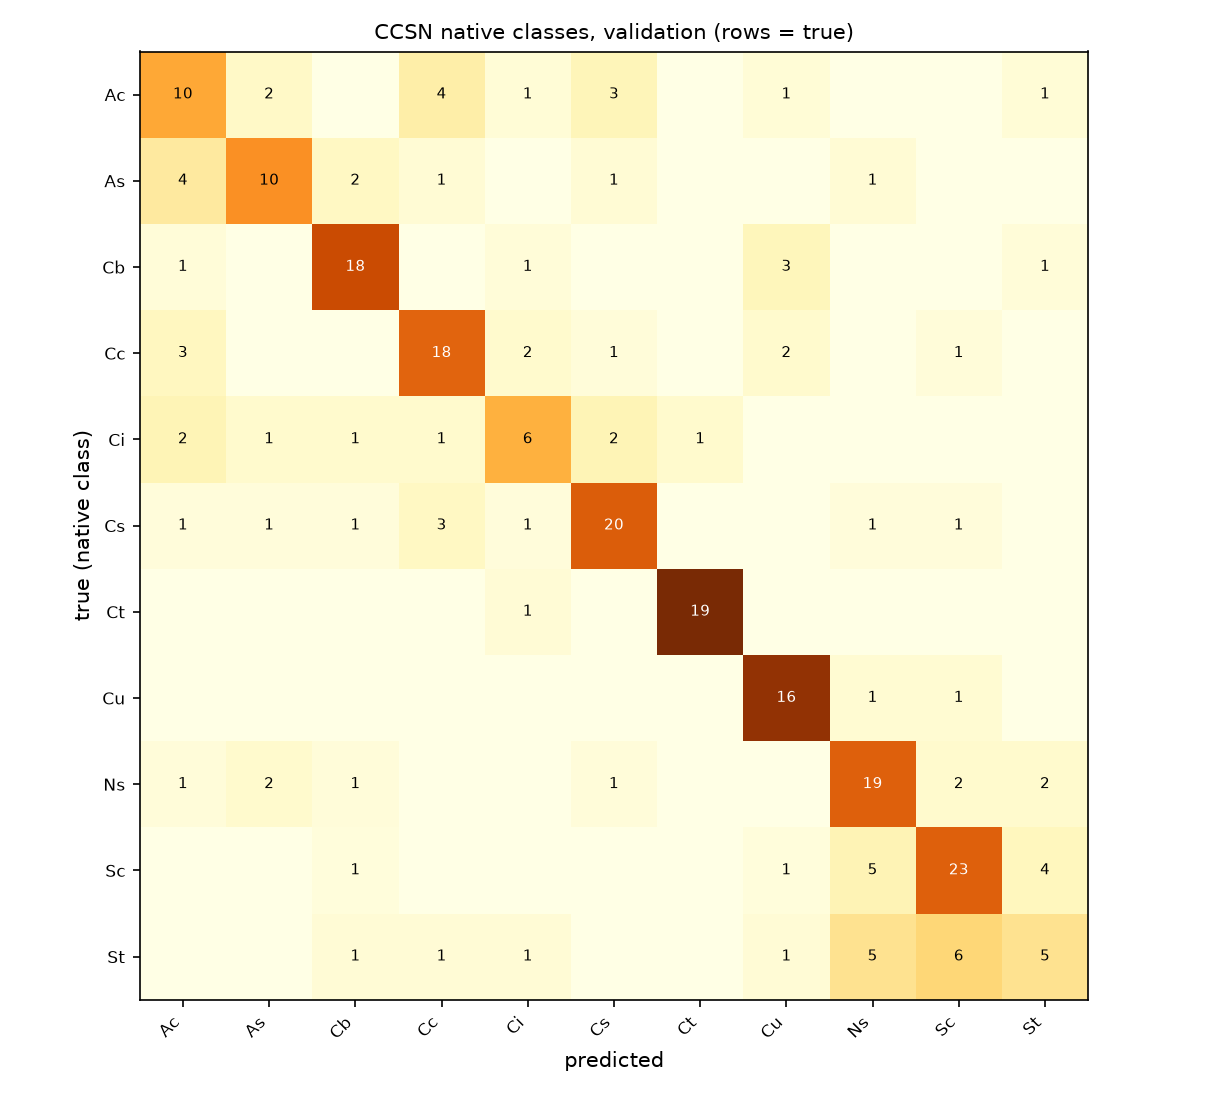
\includegraphics[width=0.9\linewidth]{supp/fig/genus_confusion_ccsn.png}
\caption{CCSN}
\end{figure}

\begin{figure}[h]
\centering
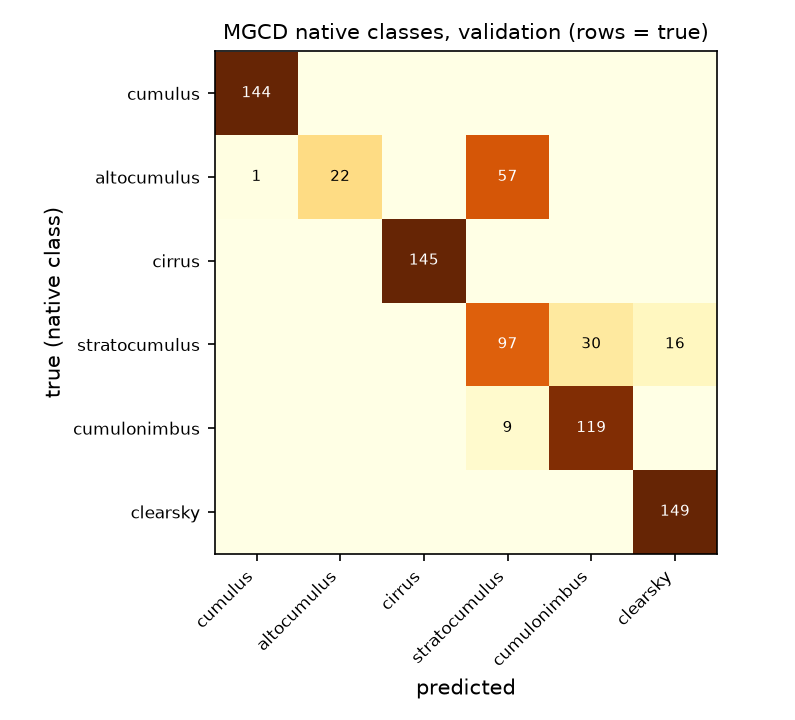
\includegraphics[width=0.9\linewidth]{supp/fig/genus_confusion_mgcd.png}
\caption{MGCD}
\end{figure}

\begin{center}{\scriptsize\setlength{\tabcolsep}{3pt}
\begin{tabular}{lllll}
\toprule
Dataset & Class & Recall & n & Most confused with (share) \\
\midrule
CCSN & all & accuracy 0.643 & 255 &  \\
CCSN & Ac & 0.455 & 22 & Cc (0.18) \\
CCSN & As & 0.526 & 19 & Ac (0.21) \\
CCSN & Cb & 0.750 & 24 & Cu (0.12) \\
CCSN & Cc & 0.667 & 27 & Ac (0.11) \\
CCSN & Ci & 0.429 & 14 & Cs (0.14) \\
CCSN & Cs & 0.690 & 29 & Cc (0.10) \\
CCSN & Ct & 0.950 & 20 & Ci (0.05) \\
CCSN & Cu & 0.889 & 18 & Ns (0.06) \\
CCSN & Ns & 0.679 & 28 & St (0.07) \\
CCSN & Sc & 0.676 & 34 & Ns (0.15) \\
CCSN & St & 0.250 & 20 & Sc (0.30) \\
MGCD & all & accuracy 0.857 & 789 &  \\
MGCD & cumulus & 1.000 & 144 &  \\
MGCD & altocumulus & 0.275 & 80 & stratocumulus (0.71) \\
MGCD & cirrus & 1.000 & 145 &  \\
MGCD & stratocumulus & 0.678 & 143 & cumulonimbus (0.21) \\
MGCD & cumulonimbus & 0.930 & 128 & stratocumulus (0.07) \\
MGCD & clearsky & 1.000 & 149 &  \\
\bottomrule
\end{tabular}}
\end{center}

\begin{center}{\scriptsize\setlength{\tabcolsep}{3pt}
\begin{tabular}{llp{12.6cm}ll}
\toprule
Dataset & Pair & Swapped share of the pair's rows & n & Counts \\
\midrule
CCSN & St/Sc & 0.185 & 54 & 6 St-$>$Sc, 4 Sc-$>$St \\
CCSN & Ci/Cs & 0.070 & 43 & 2 Ci-$>$Cs, 1 Cs-$>$Ci \\
CCSN & As/Ns & 0.064 & 47 & 1 As-$>$Ns, 2 Ns-$>$As \\
\bottomrule
\end{tabular}}
\end{center}

\subsection{Étage presence per source (exhaustive étage rows, threshold 0.5)}

\begin{center}{\scriptsize\setlength{\tabcolsep}{3pt}
\begin{tabular}{llllll}
\toprule
Source & Étage & True rate & Predicted rate & Missed & Spurious \\
\midrule
almeria & low & 0.429 & 0.583 & 0.111 & 0.354 \\
almeria & mid & 0.464 & 0.321 & 0.410 & 0.089 \\
almeria & high & 0.321 & 0.250 & 0.222 & 0.000 \\
almeria & exact set & 0.607 &  &  &  \\
ccsn & low & 0.386 & 0.407 & 0.110 & 0.103 \\
ccsn & mid & 0.263 & 0.212 & 0.355 & 0.057 \\
ccsn & high & 0.267 & 0.267 & 0.175 & 0.064 \\
ccsn & exact set & 0.771 &  &  &  \\
mgcd & low & 0.329 & 0.329 & 0.000 & 0.000 \\
mgcd & mid & 0.000 & 0.000 & 0.000 & 0.000 \\
mgcd & high & 0.331 & 0.331 & 0.000 & 0.000 \\
mgcd & exact set & 1.000 &  &  &  \\
montenegro & low & 0.609 & 0.591 & 0.051 & 0.035 \\
montenegro & mid & 0.022 & 0.020 & 0.455 & 0.008 \\
montenegro & high & 0.057 & 0.102 & 0.241 & 0.062 \\
montenegro & exact set & 0.892 &  &  &  \\
\bottomrule
\end{tabular}}
\end{center}

\subsection{Sun glare}

\begin{center}{\scriptsize\setlength{\tabcolsep}{3pt}
\begin{tabular}{lp{12.3cm}ll}
\toprule
Where & Quantity & Value & Clean \\
\midrule
val (P088 corruption) & etage\_f1: clean -$>$ sun glare & 0.760 & 0.838 \\
val (P088 corruption) & genus\_f1: clean -$>$ sun glare & 0.656 & 0.703 \\
val (P088 corruption) & sky\_miou: clean -$>$ sun glare & 0.816 & 0.901 \\
val (P088 corruption) & clear\_sky\_cloud\_fraction: clean -$>$ sun glare & 0.467 & 0.292 \\
val (P088 corruption) & cbh\_mae\_m: clean -$>$ sun glare & 745.508 & 605.748 \\
b0268 (adaptation days) & glare\_fraction\_strong\_frames & 0.000 & - \\
b0268 (adaptation days) & glare\_fraction\_other\_frames & 0.000 & - \\
\bottomrule
\end{tabular}}
\end{center}

\subsection{Failure gallery}

The validation frames with the largest étage error (exhaustive étage rows), true and predicted étages under each frame.

\begin{figure}[h]
\centering
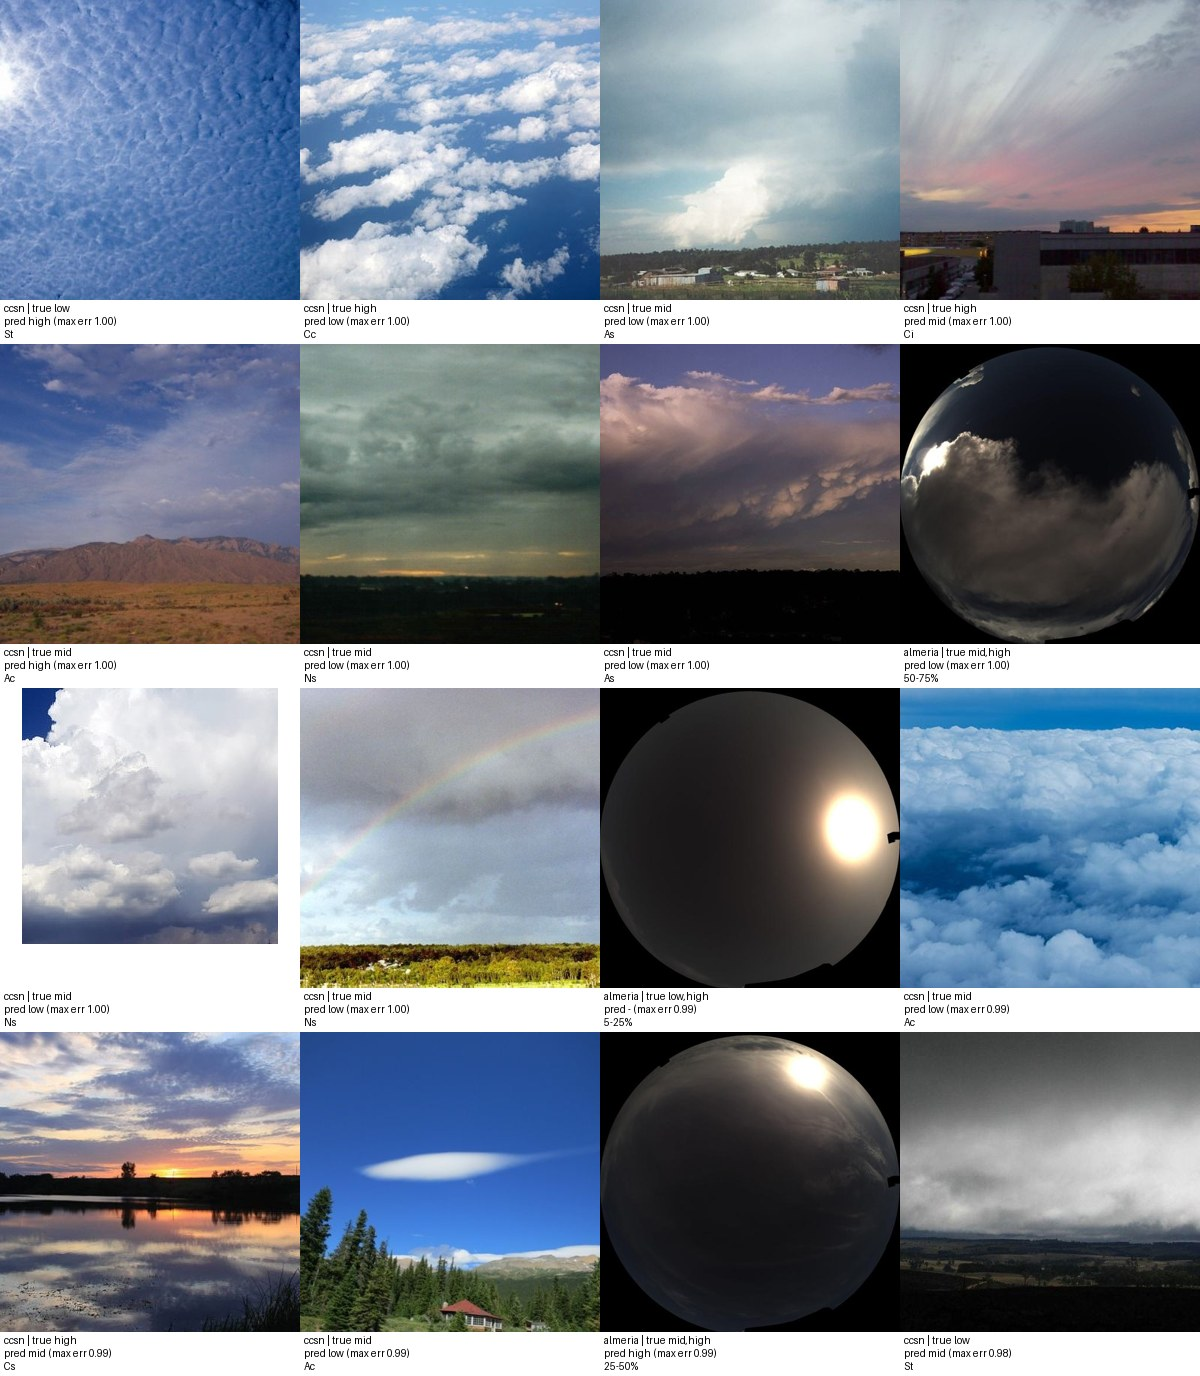
\includegraphics[width=0.9\linewidth]{supp/fig/failure_gallery.jpg}
\caption{gallery}
\end{figure}

\subsection{Dataset identity from the model's features (P029 re-check)}

\begin{center}{\scriptsize\setlength{\tabcolsep}{3pt}
\begin{tabular}{p{4.0cm}p{7.2cm}llll}
\toprule
Features & Datasets & Accuracy & Chance & n test & Note \\
\midrule
model pooled features (512-d) & eye2sky\_cbh, mgcd, montenegro, ccsn, almeria, swimcat & 1.000 & 0.167 & 131 & balanced accuracy 1.000 \\
backbone CLS features (384-d) & eye2sky\_cbh, mgcd, montenegro, ccsn, almeria, swimcat & 1.000 & 0.167 & 131 & balanced accuracy 1.000 \\
\bottomrule
\end{tabular}}
\end{center}

Attention maps were not produced: the heads pool an 8 $\times$ 8 token grid through a learned attention pool whose weights are not stored at inference; the sky-parse mask is the per-pixel view the paper shows instead.


\section{The model as a sixth annotator}

The Gate G4 global heads (\texttt{indomain\_\allowbreak{}e2s}, EMA) answer the 511 Montenegro validation images the way the 5 human raters did: an étage set from the altitude class and a cover in oktas. Krippendorff's alpha over the raters with and without the model, and each rater against the majority (étage set) or the median within $\pm$1 okta (cover) of the others, as in P035. Validation units only; the locked test is P090. Run \texttt{20261105T135320Z\_\allowbreak{}human\_\allowbreak{}ceiling\_\allowbreak{}model\_\allowbreak{}2500933325}.

\begin{center}{\scriptsize\setlength{\tabcolsep}{3pt}
\begin{tabular}{lp{13.5cm}ll}
\toprule
Quantity & Metric & Value & n \\
\midrule
étage set & alpha, humans only & 0.659 &  \\
étage set & alpha, humans + STRATIA & 0.684 &  \\
étage set & leave-one-out agreement, STRATIA vs the others' majority & 0.932 & 486 \\
étage set & leave-one-out agreement, humans (mean over raters) & 0.893 & 2047 \\
étage set & leave-one-out agreement, humans (min / max) & 0.827 / 0.955 &  \\
étage set & pairwise agreement, model-human (mean over raters) & 0.829 &  \\
étage set & pairwise agreement, human-human (mean over pairs) & 0.769 &  \\
oktas 0-8 & alpha, humans only & 0.960 &  \\
oktas 0-8 & alpha, humans + STRATIA & 0.956 &  \\
oktas 0-8 & leave-one-out agreement, STRATIA vs the others' majority & 0.892 & 509 \\
oktas 0-8 & leave-one-out agreement, humans (mean over raters) & 0.909 & 2245 \\
oktas 0-8 & leave-one-out agreement, humans (min / max) & 0.808 / 0.964 &  \\
oktas 0-8 & pairwise agreement, model-human (mean over raters) & 0.857 &  \\
oktas 0-8 & pairwise agreement, human-human (mean over pairs) & 0.874 &  \\
\bottomrule
\end{tabular}}
\end{center}

\begin{figure}[h]
\centering
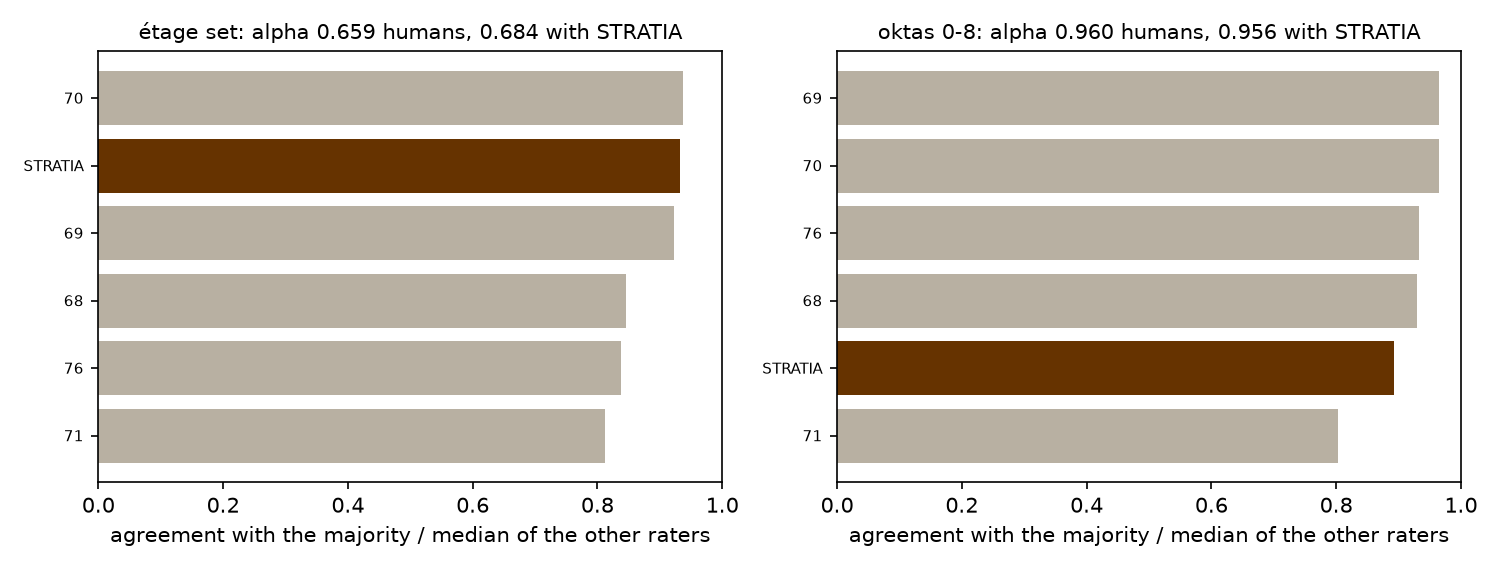
\includegraphics[width=0.9\linewidth]{supp/fig/human_ceiling_model.png}
\caption{raters}
\end{figure}

Reading: alpha is a chance-corrected agreement over the whole panel; adding a rater who agrees with the panel about as often as the humans do leaves it unchanged, a rater who disagrees systematically lowers it. The leave-one-out rows put the model on the same footing as each human: its agreement with the others' majority next to theirs.


\section{Calibration}

Per-head temperatures fitted on one half of the validation units and scored on the other (both ways); the parameters in \texttt{configs/calibration.json} are fitted on all validation rows. ECE with 15 bins. The locked test sets are not read.

\subsection{Global heads}

\begin{center}{\scriptsize\setlength{\tabcolsep}{3pt}
\begin{tabular}{lp{6.3cm}lllp{5.2cm}l}
\toprule
Head & Quantity & n & ECE before & ECE after & Temperature (cross-fit mean / all-val) & Applied \\
\midrule
genus & ECE of the predicted native class (CCSN, MGCD) & 1214 & 0.145 & 0.092 & 3.71 / 4.49 & yes \\
etage & ECE (Bernoulli, exhaustively labelled rows) & 3891 & 0.023 & 0.045 & 1.38 / 1.24 & no (T = 1) \\
oktas & ECE (top class vs majority) & 511 & 0.030 & 0.092 & 0.43 / 0.65 & no (T = 1) \\
\bottomrule
\end{tabular}}
\end{center}

\subsection{CBH head}

\begin{center}{\scriptsize\setlength{\tabcolsep}{3pt}
\begin{tabular}{p{12.1cm}lll}
\toprule
Quantity & Raw & Temperature & Temperature + conformal \\
\midrule
80 \% interval coverage (cross-fit) & 0.874 & 0.910 & 0.798 \\
95 \% interval coverage (cross-fit) & 0.966 & 0.986 & 0.952 \\
MAE of the median (m, cross-fit) & 561 & 562 & 562 \\
\bottomrule
\end{tabular}}
\end{center}

CBH temperature 1.24 (cross-fit mean 1.24); conformal radii 0.326 (80 \%) and 0.438 (95 \%) in CDF units on 1368 cloudy validation pairs.

\subsection{OOD threshold}

\texttt{OodScore} refitted on the trained global head (pooled feature + genus logits, 6,000 training rows); threshold 1.457 = the 95th percentile of in-domain validation scores (flags 5.0\% of them by construction) flags 25.3\% of 1,500 SWIM segmentation patches (AUROC 0.928).

Parameters: \texttt{configs/calibration.json} (model-card \texttt{calibration.temperatures}, \texttt{ood\_\allowbreak{}threshold}).


\section{Robustness}

Stage H candidates on corrupted validation images, backbone run live: 1200 recognition rows (CCSN, MGCD, Montenegro, Almería), 400 segmentation images, 100 clear-sky Eye2Sky frames, 800 CBH pairs. Each cell: metric under the corruption (change vs clean in brackets).

{\scriptsize\setlength{\tabcolsep}{3pt}
\begin{longtable}{lllllll}
\toprule
Corruption & Mean étage F1 & Genus F1 (CCSN, MGCD) & Sky mIoU & Clear-sky cloud fraction & CBH MAE (m) & CBH skill \\
\midrule
\endhead
clean & 0.838 & 0.703 & 0.901 & 0.292 & 606 & +0.446 \\
exposure x0.6 & 0.830 (-0.008) & 0.708 (+0.004) & 0.899 (-0.002) & 0.306 (+0.014) & 611 (+6) & +0.441 (-0.005) \\
exposure x1.5 & 0.822 (-0.016) & 0.694 (-0.010) & 0.900 (-0.001) & 0.312 (+0.019) & 602 (-4) & +0.450 (+0.004) \\
haze 40\% & 0.817 (-0.022) & 0.713 (+0.010) & 0.893 (-0.008) & 0.308 (+0.016) & 664 (+58) & +0.393 (-0.053) \\
dirty lens & 0.804 (-0.034) & 0.635 (-0.068) & 0.893 (-0.008) & 0.308 (+0.016) & 608 (+2) & +0.445 (-0.002) \\
sun glare & 0.760 (-0.078) & 0.656 (-0.048) & 0.816 (-0.085) & 0.467 (+0.174) & 746 (+140) & +0.318 (-0.128) \\
jpeg q30 & 0.812 (-0.026) & 0.729 (+0.025) & 0.894 (-0.007) & 0.207 (-0.086) & 779 (+174) & +0.288 (-0.159) \\
sensor noise & 0.741 (-0.098) & 0.678 (-0.026) & 0.848 (-0.053) & 0.258 (-0.034) & 1014 (+408) & +0.073 (-0.373) \\
blur 2px & 0.806 (-0.032) & 0.680 (-0.024) & 0.895 (-0.006) & 0.246 (-0.046) & 742 (+137) & +0.321 (-0.125) \\
\bottomrule
\end{longtable}}

Rows in \texttt{data/robustness.parquet}. Corruptions follow the P048 photometric functions where one exists.


\section{Efficiency}

The deployed graph (\texttt{models\textbackslash\{\}stratia-1.0.1-demo\textbackslash\{\}stratia.onnx}, 512 x 512 input), run \texttt{20261105T141627Z\_\allowbreak{}efficiency\_\allowbreak{}578b90289f} on the laptop.

\subsection{Parameters}

\begin{center}{\scriptsize\setlength{\tabcolsep}{3pt}
\begin{tabular}{p{15.6cm}l}
\toprule
Component & Parameters \\
\midrule
backbone (DINOv3 ViT-S/16, frozen) & 21.597 M \\
SkyRay encoder, global & 0.101 M \\
global heads & 0.996 M \\
SkyRay encoder, CBH & 0.101 M \\
CBH head & 0.206 M \\
dense heads & 0.355 M \\
OOD score (buffers) & 0.263 M \\
total trainable above the backbone & 1.760 M \\
total & 23.356 M \\
\bottomrule
\end{tabular}}
\end{center}

FLOPs per frame (one forward pass at 512 x 512): \textbf{45.7 GFLOPs}, of which the backbone 44.3 GFLOPs; everything above the backbone costs 1.40 GFLOPs.

\subsection{Latency}

\begin{center}{\scriptsize\setlength{\tabcolsep}{3pt}
\begin{tabular}{p{8.7cm}lllp{5.2cm}}
\toprule
Setting & Median ms & p95 ms & Runs & Note \\
\midrule
pytorch fp32, RTX 4050, batch 1 & 19.5 & 23.7 & 20 &  \\
pytorch autocast fp16, RTX 4050, batch 1 & 15.0 & 16.2 & 20 &  \\
pytorch fp32, RTX 4050, batch 8 (per frame) & 16.5 & 16.5 & 10 &  \\
onnx runtime CPU, batch 1 & 144.1 & 149.4 & 10 &  \\
the desktop application ONNX Runtime DirectML (NVIDIA GeForce RTX 4050 Laptop GPU), batch 1 & 29.2 & 33.0 & 20 & preprocess 29 ms (host resize of a 16 MP frame) \\
the desktop application ONNX Runtime CPU, batch 1 & 148.7 & 153.7 & 20 & preprocess 29 ms (host resize of a 16 MP frame) \\
Raspberry Pi 5 & --- & --- & --- & not measured: no Raspberry Pi 5 on hand \\
\bottomrule
\end{tabular}}
\end{center}

GPU: NVIDIA GeForce RTX 4050 Laptop GPU; CPU: Intel64 Family 6 Model 183 Stepping 1, GenuineIntel. The the desktop application rows come from \texttt{cloudscope-aibench} (ONNX Runtime 1.24 inside the desktop application) and are the numbers the demo runs at; the PyTorch rows are the research model without export. NFR-PERF-05 (the desktop application) asks for the latency targets here.


\section{The authors' camera: Sun track and pose}

The Sun found in every logged frame (brightest saturated plateau within 25$^\circ$ of the ring of the Sun's zenith angle under the declared zenith pointing; quarter-resolution decode, 31-px window) as a camera-frame ray through the nominal fisheye model of P042, fitted against the sidecars' Sun vectors with P044's trimmed Kabsch. The declared pointing is the identity rotation; its residual is what the P083/P084/P090 ray maps carried.

{\tiny\setlength{\tabcolsep}{3pt}
\begin{longtable}{llllllllll}
\toprule
Days & Frames & Detections & Inliers & Span (h) & Declared median / p90 ($^\circ$) & Fitted median / p90 ($^\circ$) & Roll / pitch / yaw ($^\circ$) & Yaw by azimuth difference, median (IQR) & Status \\
\midrule
\endhead
all & 273 & 269 & 267 & 71.9 & 106.80 / 126.29 & 9.08 / 15.98 & -4.3 / 12.1 / 161.9 & 210.1 (26.1) & insufficient \\
2026-10-18 & 120 & 116 & 116 & 1.0 & 123.21 / 128.64 & 5.93 / 10.73 & not identifiable (arc $<$ 3 h) & 221.3 (7.2) & insufficient \\
2026-10-19 & 120 & 120 & 118 & 1.0 & 98.62 / 108.31 & 9.44 / 16.19 & not identifiable (arc $<$ 3 h) & 201.8 (15.2) & insufficient \\
2026-10-21 & 33 & 33 & 26 & 1.7 & 69.14 / 100.81 & 3.25 / 8.19 & not identifiable (arc $<$ 3 h) & 185.0 (12.3) & insufficient \\
\bottomrule
\end{longtable}}

Status rule (P044): inliers $\geq$ 15, span $\geq$ 3.0 h, median $\leq$ 1.0$^\circ$, p90 $\leq$ 2.0$^\circ$ on the inliers. The nominal model is the datasheet fisheye (f = 2540.7 px, no measured distortion), and the detector takes the centre of a saturated plateau that can span 40$^\circ$ of sky, so a residual well above the Eye2Sky 0.1$^\circ$ says 'intrinsics and detector' as much as 'pose'; the yaw is the robust part (it only needs the Sun's azimuth in the picture).

\subsection{Focal scale}

The fit with the nominal focal length scaled. The residual falls slowly as the focal grows while the inferred axis tilt grows with it: focal and tilt are degenerate under this detector, so the scan is a diagnostic and the nominal focal is kept; a checkerboard calibration (P031) is what resolves it.

{\scriptsize\setlength{\tabcolsep}{3pt}
\begin{longtable}{llllll}
\toprule
Focal $\times$ & n & Median ($^\circ$) & p90 ($^\circ$) & Yaw ($^\circ$) & Axis elevation ($^\circ$) \\
\midrule
\endhead
0.8 & 269 & 11.04 & 18.59 & 161.0 & 86.5 \\
0.9 & 269 & 9.98 & 16.89 & 161.7 & 82.2 \\
1.0 & 269 & 9.08 & 15.98 & 161.9 & 77.1 \\
1.1 & 269 & 8.62 & 14.89 & 162.0 & 72.9 \\
1.2 & 269 & 8.19 & 14.24 & 161.8 & 69.3 \\
1.3 & 269 & 7.88 & 13.63 & 161.6 & 66.2 \\
1.5 & 269 & 7.29 & 12.75 & 160.9 & 61.2 \\
\bottomrule
\end{longtable}}

\begin{figure}[h]
\centering
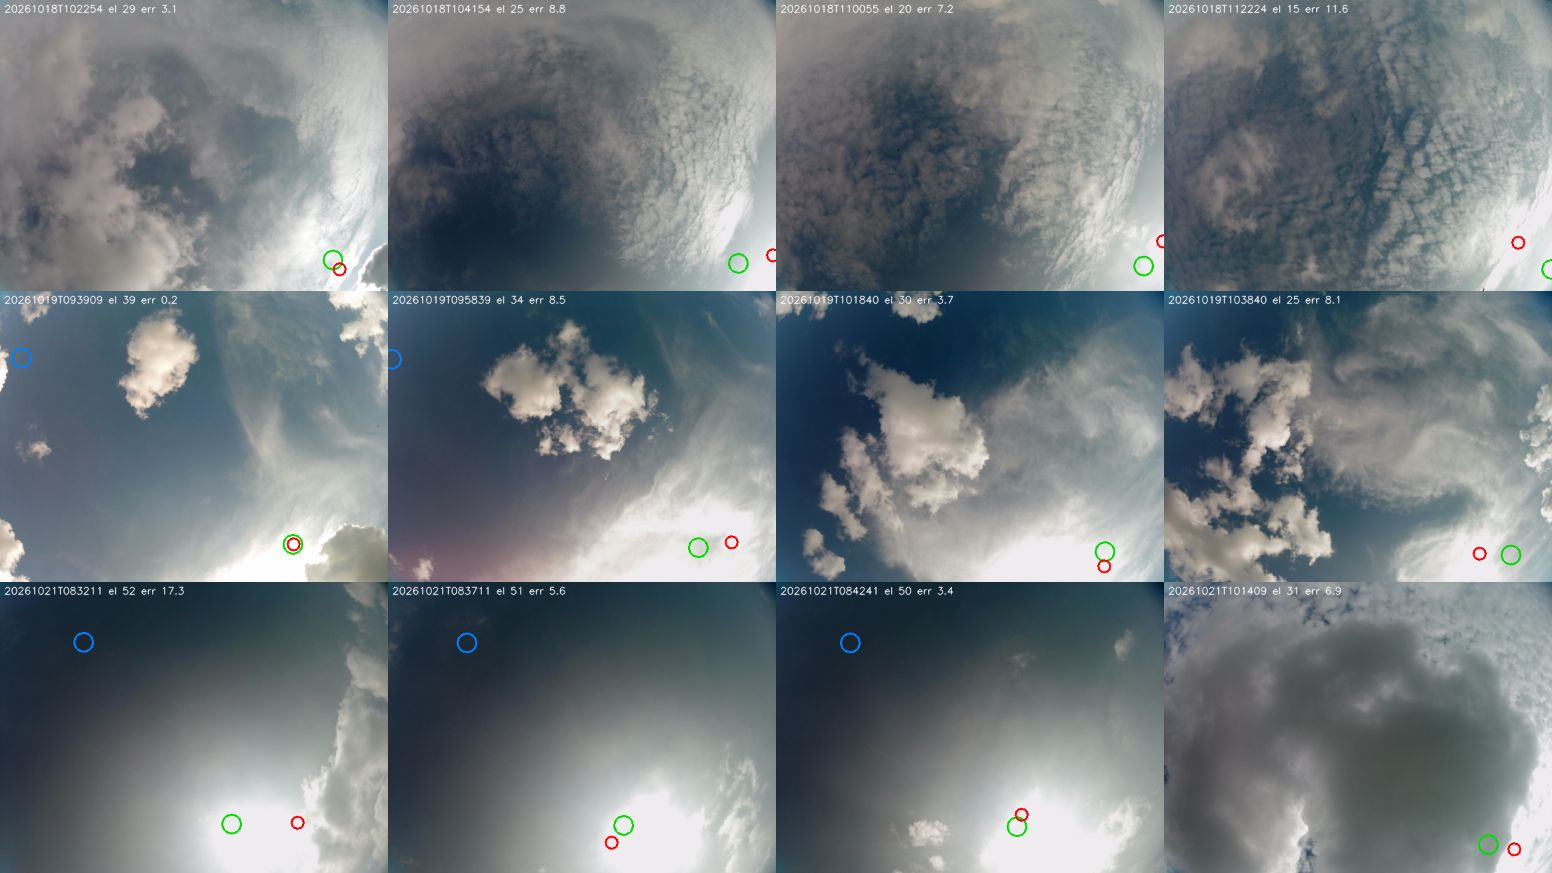
\includegraphics[width=0.9\linewidth]{supp/fig/b0268_sun_track.jpg}
\caption{detections against the declared and fitted poses}
\end{figure}

Twelve frames, four per day: red = detected plateau, blue = the Sun under the declared identity pose (off the glare in every frame), green = under the fitted pose.

Rows in \texttt{data/b0268\_sun\_track.parquet}; the pose record \texttt{BLR01\_b0268\_nominal} in \texttt{configs/camera\_poses.yaml} (nothing reads it yet: the P083/P084 ray maps and the locked-day evaluation used the declared identity pose and stay as reported).


\section{Data card}

Written in the spirit of \emph{Datasheets for Datasets} (Gebru et al.) for the collection of public sky-camera datasets and our own captures that STRATIA trains and evaluates on. Every number below comes from a Stage C report under \texttt{docs/data/}; the card is the sign-off of that audit. Date: 2026-10-08. Manifest: \texttt{data/manifest.parquet}, 52,032 rows, \texttt{sample\_id} content hash \texttt{464078b6d033dd39} (first 16 hex digits of SHA-256 over the ordered ids).

\subsection{1. Motivation}

STRATIA is a single-camera sky-understanding model (cloud genus and étage, total cover, sky parsing, cloud-base height) meant to transfer across cameras. The collection exists to (a) train and evaluate that model with a protocol in which leakage, shortcuts and label noise are measured rather than assumed away, and (b) serve as a leakage-audited, WMO-harmonised benchmark (Paper A). It was assembled by the STRATIA author (undergraduate, Bengaluru) with the AI assistant that wrote this repository; no funding.

\subsection{2. Composition}

{\scriptsize\setlength{\tabcolsep}{3pt}
\begin{longtable}{lllllll}
\toprule
Source & Images & Camera & Labels shipped & Time span & Site & Licence \\
\midrule
\endhead
Eye2Sky (AURIC, BARSE) & 29,288 & fisheye all-sky, 2,112 px, 30 s & none (ceilometer targets at other stations) & 1–9 Apr 2022 in the manifest (Apr–Jul on disk) & Oldenburg region, DE & CDLA-Sharing-1.0 \\
SWIM family: SWIMSEG 1,013, SWINSEG 115, SWINySEG 6,768, SWIMCAT 784, SHWIMSEG 156 & 8,836 & WSI crops and patches, 125–600 px & binary sky/cloud masks; SWIMCAT 5 categories & undated & Singapore & CC-BY-NC-4.0 \\
MGCD & 8,000 & fisheye all-sky, 1,024 px & 7 sky types, official 4,000/4,000 split & undated & Tianjin, CN & research use by agreement \\
CCSN & 2,543 & consumer photographs, 256–400 px & 11 classes (10 genera + contrail) & undated & web & CC0-1.0 \\
Montenegro & 2,522 & fixed low-cost camera, 640 px, 20 min & 5–9 raters: altitude class, N, Nh, h, CL, CM, CH & 3 Oct – 17 Dec 2025 & Montenegro & CC-BY-4.0 \\
Almería (DLR) & 818 & fisheye all-sky, 512 px (Kontas + 3 test cameras) & 5-class masks (camera, sky, low, mid, high); official train/val/test & 2017–2021 (file names) & PSA Almería, ES & CC-BY-4.0 \\
B0268 (ours) & 418 & Arducam B0268 fisheye USB, 4656 x 3496, zenith mount: 25 legacy frames + 393 sky-logger frames at 30 s & image-level labels on the 393 logged frames by the P041 annotator pair (A, B; language models, not human labellers) with sheets C, D for sensitivity; none on the legacy frames & 27 Sep 2026 (legacy); 18–21 Oct 2026, four afternoons (logged) & Bengaluru, IN (BLR01) & authors \\
Ceilometers CDLRA, CDLRB & 1,359,329 records & Lufft CHM15k, 15 s & lowest base, layers, flags & Apr–Jul 2022, 118 days each & Oldenburg region, DE & CDLA-Sharing-1.0 \\
\bottomrule
\end{longtable}}

Totals: 11 image sources, 6 camera types, 52,032 images, 1.36 M ceilometer records (P041, 2026-10-22: the 393 logged B0268 frames are appended to the manifest after the 52,032 locked rows, 52,425 in all). Not obtained: DeepSky and WEBCAM (authorss asked, no reply), HBMCD and GRSCD (Baidu links not reachable), LenghuSky-8 labels; GRSCD is treated as the same source as MGCD (P028).

\textbf{What is in the images besides sky.} Fixed structure (fisheye corners, horizon objects, mounts) covers 36–37 \% of an Eye2Sky frame, 25 \% of MGCD, 26 \% of Almería; Eye2Sky carries a burned-in text block (top left), Montenegro a timestamp and a logo (\texttt{docs/data/shortcuts\_report.md}, masks in \texttt{cache/features/camera\_stats\_224.npz}).

\textbf{Label distributions} (\texttt{docs/data/imbalance\_report.md}): class sets are nearly balanced (largest/smallest 2–3); Montenegro is 58 \% low cloud with raters almost never above 1.5 km and U-shaped oktas; the segmentation sets hold 1.4 \% clear and 2.7 \% overcast frames; ceilometer records are 34 \% "no cloud overhead", 34 \% low, 20 \% mid, 12 \% high.

\subsection{3. Collection process}

Public sources were downloaded from their official records (Zenodo, GitHub, institutional pages; URLs and licence checks in \texttt{configs/datasets.yaml}, \texttt{docs/data/acquisition.md}). Eye2Sky images for stations AURIC and BARSE were downloaded for April–July 2022; the manifest ingests 1–9 April (nine days per station) to keep the audit and the image cache tractable; the two ceilometer stations (CDLRA at OLDLR, CDLRB at WESTE) have \textbf{no images on disk}, so no image–ceilometer pair exists yet (open item, Paper B). B0268 frames are the 25 legacy captures of the the desktop application project plus the 393 frames its sky logger wrote over four afternoons (18–21 Oct 2026; P041), each with a JSON sidecar. Timestamps: Eye2Sky from file names (UTC), Montenegro from local time stated as UTC+1 (daylight saving not verified), Almería from file names (time zone not stated, taken as UTC; no sun position derived), legacy B0268 from EXIF (assumed UTC+5.5 h), logged B0268 from the sidecars (UTC, site, Sun, pointing).

\subsection{4. Preprocessing, cleaning, labelling}

\begin{itemize}
\item \textbf{Cache:} every image decoded once and stored at a longest side of 768 px (\texttt{cache/img768}, 3.16 GB); models read the cache (P022).
\item \textbf{Integrity (P023):} all 52,032 images decode; no corrupt, empty, mis-sized, rotated or odd-mode file; 43 featureless clear-sky patches flagged "blank" and kept. \texttt{docs/data/integrity\_report.md}.
\item \textbf{Exact duplicates (P024):} 661 images in 312 within-dataset groups (SWINySEG 533, SWIMSEG 52, CCSN 34, SWIMCAT 34, SHWIMSEG 6, Almería 2), none across datasets; one \texttt{group\_id} per group at split time. \texttt{docs/data/duplicates\_report.md}.
\item \textbf{Near-duplicates (P025):} copies (dihedral pHash $<$= 2) and same scenes (DINOv3 cosine $>$= 0.97): 14,112 images in 1,656 groups; \textbf{34.6 \% of SWINySEG are flipped, rotated or re-encoded copies of SWIMSEG/SWINSEG}; MGCD's 8,000 images are about 227 scenes. The SWIM family is one source. \texttt{docs/data/near\_duplicates\_report.md}.
\item \textbf{Label conflicts (P026):} 7.9 \% of CCSN images carry a second genus on a copy of themselves; MGCD labels are per sequence; Montenegro raters reach no majority on cloud height for 39 \% of images; SWIMSEG images annotated twice agree on 95 \% of pixels. Policy: flag, never auto-correct; conflicting pictures never in a test split; training labels decided by the harmonisation. \texttt{docs/data/label\_conflicts\_report.md}.
\item \textbf{Temporal structure (P027):} Eye2Sky frames are the same scene 82–92 \% of the time at 30 s and reach the different-day level after 8.5–17 h (block = calendar day); Montenegro stays correlated across days (block = 7-day run); Almería day blocks; the two Eye2Sky stations are correlated but not duplicates. \texttt{docs/data/temporal\_report.md}.
\item \textbf{Shortcuts (P029):} the dataset is readable from frozen features at 99.7 \%, the Eye2Sky station at 100 \% from the sky alone, the hour of day at 4–6$\times$ chance; Montenegro's text strip predicts its class above chance. Mitigations: out-of-camera protocol, per-camera masks, resolution normalisation, explicit sun input. \texttt{docs/data/shortcuts\_report.md}.
\item \textbf{Ceilometer (P014, P031):} streams 99.998 \% complete; 3.5–6.1 \% of records flagged (rain, window, optics, errors); CDLRA's laser-ageing bit on 58 \% of records is a warning, not an error; pairing tolerance $\pm$30 s. \texttt{docs/data/ceilometer\_qc.md}.
\item \textbf{Labels (Stage D):} \texttt{configs/ontology.yaml} maps every native class to WMO genus sets or excludes it (P033); mapping, soft labels, ceilometer targets, splits and the test lock follow in P034–P039.
\end{itemize}

\subsection{5. Uses}

Intended: training and evaluating single-camera sky understanding with the protocol of \texttt{docs/research\_design.md}: leave-one-dataset-out and held-out-station tests, day- or week-blocked splits, square-root source sampling and class-balanced losses (P030), macro metrics with per-source and per-sun-zenith reporting, CBH scored against the ceilometer at the same site only (a cloud base 15 km away differs by 255 m at the median and disagrees on presence 18 \% of the time). Not intended: pooled accuracies over mixed sources without per-source numbers (they measure "which camera"); any claim about genera for SWIMCAT (appearance categories only); training a general cloud-height model on Montenegro's height code (local, low-cloud, no majority for 39 \% of images); any use of the SWIM family beyond non-commercial research (CC-BY-NC); commercial use of MGCD without its agreement.

\subsection{6. Distribution}

STRATIA redistributes no images. The repository holds code, manifests of file paths, derived tables (hashes, groups, flags, splits) and figures; the figures derived from Eye2Sky are shared under CDLA-Sharing-1.0 terms. B0268 frames are the authors'; their EXIF GPS is rounded to 0.01$^\circ$ in any published form (open decision on the legacy public frames). Model weights trained on this collection inherit the most restrictive licence of their training sources (CC-BY-NC for anything that saw the SWIM family).

\subsection{7. Maintenance}

Maintained in the STRATIA repository by its author; versioned by the manifest content hash above, the per-phase documents under \texttt{docs/phases/}, and the test-set lock (P039). Changes to the collection are new phases with new reports, never silent edits of labels or files.

\subsection{8. Known limitations and open items}

{\scriptsize\setlength{\tabcolsep}{3pt}
\begin{longtable}{llll}
\toprule
Item & Effect & Owner / phase & Blocks G1? \\
\midrule
\endhead
No images at the ceilometer sites (OLDLR, WESTE) & no image–CBH pairs; Paper B training impossible until downloaded & authors download; P036 (targets ready), P047 (pairing) & no (Paper A unaffected) \\
Manifest holds 9 of \textasciitilde{}120 Eye2Sky days per station & few day blocks for Eye2Sky splits & P038 decides whether to ingest more days at a lower cadence & no \\
DeepSky, WEBCAM, HBMCD, GRSCD not obtained & fewer sources; GRSCD counted as MGCD & P015 cut-off 15 Oct & no \\
Almería and Montenegro time zones not verified; no Almería sun position & day blocks safe, hour-level analyses approximate & data card note; P044 ray maps for Almería unavailable & no \\
WMO code-table wording written from memory & appendix must be checked against WMO-No. 306 & P033 open item, before the paper & no \\
B0268 labels come from language-model annotators (P041), not the two human labellers of the plan; four days instead of six or more & OOD and adaptation numbers (P083, P084) carry that caveat; the day-blocked protocol has one locked test day & authors: human labels on a subset; P083 / P084 & no \\
CCSN label noise and cross-étage conflicts & genus scores on CCSN capped & P034 merges sets; test exclusion & no \\
\bottomrule
\end{longtable}}

\subsection{9. Gate G1 sign-off}

{\scriptsize\setlength{\tabcolsep}{3pt}
\begin{longtable}{ll}
\toprule
Check & Status \\
\midrule
\endhead
Every image decodes and matches the manifest (P023) & passed \\
Exact and near-duplicate groups defined for the splits (P024, P025) & passed \\
Label conflicts listed with a policy (P026) & passed \\
Temporal blocks decided per dataset (P027) & passed \\
Double counting across sources documented (P028) & passed (deferred measurement, policy in place) \\
Shortcut list with mitigations (P029) & passed \\
Imbalance measured, sampling chosen (P030) & passed \\
Ceilometer QC and pairing tolerance (P031) & passed \\
Blockers for Paper A & \textbf{0} \\
\bottomrule
\end{longtable}}

Signed: STRATIA author, 2026-10-08 (commit of P032). Paper B's data dependency (images at the ceilometer sites) is recorded above as an open item, not a G1 blocker.



\end{document}
